

\chapter{Структурная биоинформатика} \label{phys_sbio}

\section{Математика и физика в структурной биоинформатике} \label{sect1_1}

При работе в области структурной биоинформатики несомненно следует иметь достаточно образования в классических дисциплинах, на которых основаны современные расчетные методы. В широком смысле, эти дисциплины - теоретическая физика, включая ее математический аппарат, и вычислительная математика. В настоящем учебнике вопросы касающиеся этих дисциплин объяснены на поверхностном уровне, и в рамках этого учебника нет возможности для более углубленного их изложения. Поэтому авторы посчитали нужным вкратце упомянуть во введении темы, которые следует более внимательно изучить в этих дисциплинах, и некоторые учебные курсы, в которых они изложены.

В традициях российской научной школы, изложение теоретической физики обычно следует канве "от общего к частному", и классическим курсом по теоретической физике здесь следует назвать "курс теоретической физики" Ландау и Лифшица \parencite{Ландау_1,Ландау_2,Ландау_3,Ландау_5}. Первые части этого курса, в порядке следования, это "Механика", "Теория поля", "Квантовая механика", "Квантовая электродинамика", "Статистическая физика". Основы разделов физики, излагаемые в каждом из этих томов (кроме квантовой электродинамики), важны для понимания методов в структурной биоинформатике. 

%Разделы настоящего пособия также построены по сходной схеме.

Среди классических курсов теоретической физики, используемых в англоязычных вузах и доступных в русских переводах, следует упомянуть "Фейнмановские лекции по физике" \parencite{Фейнман_eng,Фейнман_rus}, записи лекций американского физика Ричарда Фейнмана, и "Методы теоретической физики" Филлипа Морса и Германа Фешбаха \parencite{Morse_eng,Морс_1,Морс_2}. Более широкий обзор учебных курсов по теоретической физике находится за рамками данного учебника и за рамками опыта авторов. Однако каждый из трех упомянутых курсов использует свою схему и стилистику изложения и объяснения материала, и потому не следует считать что условием вхождения в структурную биоинформатику является блестящее знание какого либо из этих учебников. Однако при работе в биоинформатике зачастую возникают вопросы, ответы на которые можно найти, только освоив материал, излагаемый в этих курсах, как, впрочем, и во многих других курсах физики.

Создание современной теоретической физики в XX веке стало возможно во многом из-за появления математического аппарата, с помощью которого стало возможным записать фундаментальные законы физики в форме точных уравнений. Среди разделов высшей математики, необходимой для полноценной работы в биоинформатике и для понимания основ теоретической физики, следует перечислить, в порядке важности, следующие темы: владение понятиями вектора и матрицы и обращения с этими объектами, излагаемое обычно в разделах аналитической геометрии и линейной алгебры; основы интегрального и дифференциального исчисления, понятие о дифференциальных уравнениях; теория функций комплексного переменного. Отдельно выделяется раздел методов теории вероятностей и математической статистики; владение этими методами необходимо при решении большей части задач современной молекулярной биологии. 

Российская школа классической математики, по наблюдениям историков науки, является одной из трех или четырех независимых и развивающихся математических традиций. Многих ученых из этой школы можно упомянуть как безусловно авторитетных для всех современных математиков, как, например, академика Колмогорова, академика Понтрягина, академика Гельфанда, и безусловно целый ряд других имен. И потому многие из курсов высшей математики на русском языке можно считать подходящими для изучения упомянутых выше разделов и предметов.

Вычислительная математика является относительно молодой наукой, она начала развиваться с 50х и 60х годов XX века. Помимо того, это прикладная наука, в ней намного меньше общих понятий и намного больше частных решений. Тем не менее в вычислительной математике сформировались некоторые общие принципы при подходах к решению задач линейной алгебры, численному решению дифференциальных уравнений и вычислению интегралов, задачам оптимизации и распознавания образов. Изложение этих принципов можно найти в учебных курсах по вычислительной математике, однако предпочтения и специализация авторов курсов в этой науке более заметны. И также, именно из вычислительной математики произошла бурно развившаяся наука о разработке программ и алгоритмов, так называемая "наука о компьютерах" (computer science). Тут, оставляя вне рамок данного пособия большую часть работ и изобретений в этой области, все же следует упомянуть классические учебники по программированию: учебник Никлауса Вирта \parencite{Wirth_eng,Вирт_1982}, разработчика языка Паскаль, учебик по языку Си Брайна Кeрнигана и Денниса Ритчи \parencite{Керниган_1992,Kernighan_1978}, учебник по языку Си++ Бьерна Страуструпа \parencite{Stroustrup_1985} - несмотря на появление все новых, более удобных, средств разработки программ, в этих учебниках можно найти некоторые общие принципы, не изменившиеся со времен появления науки о компьютерах.

С другой стороны, со времен появления информатики, технологии программирования непрерывно развиваются, появляются новые понятия, и процесс программирования становится все более легким, удобным и эффективным. Также и в смежных дисциплинах, в математической статистике, в численных методах и в теоретической физике, появляются универсальные термины, допускающие совместное использование разных подходов в этих областях. 

\begin{figure}[H]
  \centering
  \vskip 12pt 
  \includegraphics [width=0.8\linewidth]{sbhist_scheme.png}
  \vskip 12pt
  \caption[m1]{
  \textbf{Иллюстрация истории развития идей и дисциплин физики и математики, используемых в структурной биоинформатике.}\itshape

  Горизонтальная ось - шкала исторического времени. В правой части рисунка показаны темы структурной биоинформатики, обсуждаемые в пособии, и их связь с физико-математическими дисциплинами. Красные линии показывают время интенсивного обмена идеями между дисциплинами.
  
  \fontsize{11pt}{11pt}\selectfont
  Временные границы показаны с долей условности, как и ширина полос, которые обозначают интенсивность разработки дисциплины.
  Начало развития обозначенных тем структурной биоинформатики может быть сориентировано по указанным годам: 1969 - выход работы A. Pople \parencite{Hehre_1969} и начало разработки пакетов по квантовой химии; 1977 - выход работы M. Karplus \parencite{McCammmon_1977} и начало разработки пакетов по мол. динамике; 2000 - реорганизация журнала Journal of Computer-Aided Molecular Design; 1994 - начало проведения экспериментов CASP; 2001 - начало проведения экспериментов CAPRI;
}
 \label{img:sbhist_scheme}
\end{figure}

В настоящем пособии не изложен подробно материал физико-математических дисциплин и понятия молекулярной биологии, на которых основаны подходы структурной биоинформатики, и также в пособии в полном объеме не изложены и сами темы структурной биоинформатики, показанные на рисунке \ref{img:sbhist_scheme}. Ответы на многие вопросы, важные для практической работы и для глубокого понимания материала, следует искать в современных мультимедийных лекционных курсах и публикациях в международных журналах. Также, изложение этих тем можно найти в книгах и пособиях на русском языке, таких как \parencite{Холмодуров_2003}, \parencite{Хохлов_2009}, \parencite{Андрианов_2013}, \parencite{Финкельштейн_2012}, \parencite{Гуреев_2018}. Цель, поставленная при подготовке материала в пособии, состояла, напротив, в том чтобы отойти от изложения этих тем в рамках традиций, принятых в кругу профильных специалистов, и подготовить обзор наиболее важных идей в структурной биоинформатике, для акцентирования внимания читателя на моменты согласия и моменты различия в этих идеях и методах. 

\section{Уровни представления молекулярных систем}

\subsection{Уровень классической механики}

Механика, один из первых по времени создания разделов физики, строится на понятии \textit{«материальных точек»}. В молекулярных моделях, построенных на основе законов механики, атомы описываются как такие «материальные точки». В механике, для описания движения системы, используется понятие сил, действующих между точками. После того как заданы законы взаимодействия атомов, то есть силы, возможно в рамках законов механики рассчитать движение системы атомов на основе решения уравнения Ньютона.

Второй закон Ньютона, известный еще из курса физики в средней школе, выражает связь ускорения тела с действующей на него силой $F$, по формуле $F = m a$, где $m$ — масса тела. По форме это так называемое \textit{«дифференциальное уравнение»}; фактически, исчисление бесконечно малых, включающее понятие дифференцирования, зародилось и развивалось одновременно с зарождением механики как раздела физики. В этих терминах, ускорение $a$, входящее в уравнение Ньютона, является второй производной по времени от координаты тела: $a = \frac{d^2x}{dt^2} = F(x)$. Результатом решения такого дифференциального уравнения будет функция $x(t)$, траектория движения тела. 

Для решения дифференциальных уравнений, помимо законов движения, необходимо задать начальное положение системы. По правилам, выводимым в теории дифференциальных уравнений, уравнения, выраженные через вторые производные координат, требуют задания двух начальных параметров для каждой из координат. В случае уравнений молекулярной механики, для расчета траекторий необходимо задать начальные координаты и скорости всех атомов в системе.

Аналитические решения уравнений движения возможно получить только для случая взаимодействия двух тел (материальных точек). Эти решения известны из астрономии - это циклические движения планет по орбитам,  и гиперболические траектории небесных тел, ненадолго попадающих в область притяжения Солнца. В астрономии, взаимодействием планет между собой можно пренебречь для описания их орбит, и потому движения небесных тел можно свести к задаче двух тел. Для задачи трех и более тел, решения уравнений Ньютона нельзя, в общем случае, рассчитать аналитически. Однако из структуры уравнений движения можно доказать, что эти решения тоже можно свести к циклическим движениям, подобным движению планет по орбитам. Но период времени, за который происходит цикл такого движения, может быть несоизмеримо большим.

При развитии классической механики и теории дифференциальных уравнений, были разработаны изящные и эффективные способы аналитического анализа уравнений движения механических систем. Так, в астрономии, учет притяжения между планетами позволил, по малым отклонениям наблюдаемых траекторий планет, предсказать существование еще одной планеты в солнечной системе - планеты Нептун, которая затем и была обнаружена астрономами. Кометы, небесные тела, обращающиеся по эллиптическим орбитам и на лишь на малое время попадающие в область близкую к Солнцу, с древности привлекали внимание; появление кометы вносит малое, но непредсказуемое возмущение в движение небесных тел, орбиты которых иначе оставались бы безусловно неизменными. Однако молекулярные системы все же слишком сложны, чтобы использовать аналитические методы исследования уравнений движения, и эти уравнения следует решать численно. 

\begin{figure}[H]
  
  \centering
  \includegraphics [width=0.5\linewidth]{planets.jpg}

  \caption[m2]{
  \textbf{Парад планет}\itshape
  
  Парад планет - явление, когда несколько планет оказывается по одну сторону от Солнца в небольшом секторе, близко друг к другу на небесной сфере.
  
  \fontsize{11pt}{11pt}\selectfont
  Парад планет 1982 года на марке КНР (Wikipedia)
  }
 \label{img:planets}
\end{figure}


\subsection{Уровень статистической физики}

При представлении моделей молекулярной системы следует учитывать, что рассматриваемая молекулярная система является частью некоторой большей системы. Как пример отношения большей и меньшей систем, можно привести движения белковых молекул которые происходят в цитоплазме клетки. Взаимодействие молекул системы с внешней средой может быть учтено на основе статистических свойств внешней среды, следуя законам \textit{статистической физики}. 

Статистическая физика позволяет определить понятия относящиеся к усредненным характеристикам системы, когда количество частиц в системе велико (рис. \ref{img:idealgas}). Как пример, температура является такой статистической характеристикой, опосредованно выражающей среднюю энергию движения частиц в системе. Из уравнений движения замкнутой механической системы следует закон о сохранении полной энергии системы. Однако из-за взаимодействия с внешней средой полная энергия системы может изменяться. 

\begin{figure}[H]
  
  \centering
  \includegraphics [width=0.8\linewidth]{idealgas.png}

  \caption[m2]{
  \textbf{Идеальный газ - простейшая модель статистической физики}\itshape

  \fontsize{11pt}{11pt}\selectfont
  Изображение построено с помощью пакета matplotlib на языке программирования python
 }
 \label{img:idealgas}
\end{figure}

Аппарат статистической физики применим в полной мере к системам, находящимся в состоянии, близком к так называемому \textit{статистическому равновесию}. В этом случае, взаимодействие системы с внешней средой можно описать на основе \textit{распределения Больцмана}, называемого также распределением Больцмана-Гиббса. Это распределение связывает вероятность состояния системы, одного из возможных, с энергией $E$ этого состояния: $p = A \exp( -E/kT )$. Параметр $kT$ в этой формуле имеет размерность энергии и выражает связь системы с внешней средой. С учетом множителя $k$, называемого \textit{постоянной Больцмана}, значение $T$  - это температура, одинаковая в системе в во внешней среде.  

Понятие статистического равновесия связано с понятием \textit{энтропии} - меры неупорядоченности системы. Понятие упорядоченности можно пояснить, используя модель идеального газа (рис. \ref{img:idealgas}), большого количества молекул в замкнутом объеме. В каком бы из положений не находились молекулы газа в начале моделирования, по мере эволюции системы они будет все более равномерно распределены внутри этого замкнутого объема. При установлении статистического равновесия, распределение скоростей молекул может быть рассчитано на основе распределения Больцмана (рис. \ref{img:maxwell_distribution}), какие бы скорости не имели молекулы в начале моделирования.


\begin{figure}[H]
  
  \centering
  \includegraphics [width=0.7\linewidth]{maxwell_distribution.png}

  \caption[m2]{
  \textbf{Распределение скоростей молекул в идеальном газе для разных температур, выведенное на основе распределения Больцмана.}\itshape

    Горизонтальная ось отмечает скорость молекул (в метрах/сек), вертикальная ось - количество молекул с такой скоростью.
    
  \fontsize{11pt}{11pt}\selectfont
  Распределение вероятностей для скорости молекул в идеальном газе известно как распределение Максвелла.
  
  Изображение построено с помощью пакета matplotlib на языке программирования python
 }
 \label{img:maxwell_distribution}
\end{figure}

%Статистическая физика, описывающая равновесные системы, формулируется не в терминах определенного состояния системы, а в терминах ансамбля состояний, и в ней задается вероятность нахождения системы в каждом из состояний ансамбля. 

Как это подразумевалось при определении формулы Больцмана, в статистической физике рассматривается совместно совокупость состояний системы, так называемый \textit{ансамбль} состояний. Значение энтропию системы, при таком определении, будет выражаться формулой $S = - \sum_i p_i \log( p_i)$, где $p_i$ - вероятность каждого из состояний в ансамбле. Согласно \textit{второму началу термодинамики}, по мере эволюции системы величина энтропии всегда будет возрастать; введение понятия энтропии позволяет охарактеризовать процессы установления статистического равновесия, как, например, в упомянутой модели идеального газа. 

Следует отметить, что принцип возрастании энтропии системы можно ввести только совместно с понятием о влиянии внешнего окружения на процессы в системе; движение замкнутой системы будет описываться законами механики, и, в рамках уравнений механики, закон возрастания энтропии вывести нельзя. Это замечание обозначает парадоксальность и неполную согласованность всего подхода статистической физики; и, тем более, наибольший интерес для исследования представляют неуравновешенные и не полностью уравновешенные системы, где подход статистической физики неприменим в полной мере из-за несоответствия модели и объекта.

\subsection{Уровень квантовой механики}


%его точное аналитическое решение только для простейших моделей. 


%Атом водорода, сходный с системой из двух тел в классической механике, это одна из моделей, для которой уравнение Шредингера удается решить точно. 
На квантовом уровне описания, замкнутая система, как, например, система электронов в атоме, может находиться в одном из устойчивых \textit{стационарных состояний}, подобно орбитам небесных тел. Спектральные линии (рис. \ref{img:quantum_fespectrum}), при таком описании, означают переходы между квантовыми состояниями, при взаимодействии с возмущением извне - электромагнитным полем.

\begin{figure}[H]
  \centering
  \includegraphics [width=0.9\linewidth]{quantum_cspectrum.png}
  
  \vskip 12pt
  \includegraphics [width=0.9\linewidth]{quantum_fespectrum.png}
  
  \caption[Сравнение спектров углерода (вверху) и железа (внизу) в видимой области.]{
  \textbf{Сравнение спектров углерода (вверху) и железа (внизу) в видимой области.}\itshape

%Спектральные линии соответствуют переходу между квантовыми уровнями атома, при котором испускаются или поглощаются кванты света с энергией, в точности равной разнице в энергии уровней.
  
%У более сложного атома железа большее количество близко расположенных квантовых состояний, и потому на спектре железа в видимой области заметно значительно больше линий.

  \fontsize{11pt}{11pt}\selectfont
  Изображения спектральных линий скопированы из разделов проекта Wikipedia.

}
 \label{img:quantum_fespectrum}
\end{figure}

Основным уравнением квантовой механики, описывающей распределение волновых функций электронов в молекулярной системе, является уравнение Шредингера. Методы математического анализа и теория дифференциальных уравнений существенно развились к началу XX века, что и сделало возможным вывод точных уравнений для описания квантовых систем. Уравнение Шредингера является, в широком смысле, дифференциальным уравнением, обобщающим уравнения Ньютона. Его точное аналитическое решение возможно только для простейших моделей. 

Атом водорода, сходный с системой из двух тел в классической механике, это одна из моделей, для которой уравнение Шредингера удается решить точно. В отличии от орбит небесных тел, взаимодействием между электронами в атоме нельзя пренебречь. Стационарные состояния определяются совместно для всей системы электронов в атоме. Но даже для атома с двумя электронами такую задачу нельзя решить аналитически.

При определении квантового состояния используются понятие \textit{волновой функции}; в одной из возможных интерпретаций, волновая функция описывает совместное распределение электронов в пространстве. Каждому из состояний соответствует некоторое значение энергии системы; в устойчивой замкнутой системе состояния распределены по дискретным \textit{уровням энергии}. 
%Одному уровню энергии может ссответствовать несколько возможных состояний.  

При обобщении квантового описания системы, в терминах волновых функций, до масштаба макроскопических явлений, возникает необходимость ввести понятие \textit{квантовой редукции} - когда при наблюдении за квантовым объектом изменяется его состояние. Так, например, понятие электронного облака, условно, подразумевает что электроны "размазаны" по всему пространству вокруг атома, как это описывается их волновыми функциями. Однако при наблюдении за электроном, с помощью фотонов с достаточно высокой энергией, электрон оказывается локализован в одной из точек пространства в "облаке", и факт такого наблюдения приводит к изменениям во всей молекуле. В более общей интерпретации, состояния квантовой системы, без присутствия наблюдателя, могут описываться как \textit{смешанные}, когда система "размазана" или "распределена" по совокупости ее возможных состояний. Эффект наблюдения выражается в редукции системы к одному из  состояний; вероятность редукции к определенному состоянию определяется через абсолютную величину волновой функцию.


\begin{figure}[H]
  
  \centering
  \includegraphics [width=0.5\linewidth]{cat.jpg}
  \vskip 12pt
  \caption[m2]{
  \textbf{Кот Шредингера.}\itshape
  
Иллюстрация к мысленному эксперименту, описанному Шредингером и демонстрирующему парадоксальность принципов квантовой механики.
  
В этом мысленном эксперименте рассматривают черный непроницаемый для наблюдателя ящик, в который посажен живой кот. В течении эксперимента кот может погибнуть, но в рамках обобщения квантовой механики до макроскопических объектов, возможно представить смешанное квантовое состояние, сочетающее в себе живого кота и мертвого кота.
  
  \fontsize{11pt}{11pt}\selectfont
  Рисунок Михаила Малоземова.
  
 }
 \label{img:quantum_сat}
\end{figure}

Вопросы неполноты и парадоксальности квантовой механики были замечены учеными при разработке основ этой теории (рис. \ref{img:quantum_сat}). При развитии методологии и экспериментальных техник, подтвердились и углубились постановки задач, вызывавшие сомнение при создании теории. Эти эффекты привели к появлению новых направлений в физике; как пример, можно привести исследования в области \textit{квантовые компьютеры} и \textit{квантового шифрования}, связанные с понятием \textit{квантовой запутанности} (quantum entanglement). Однако даже в этой фундаментальной и математически безупречной области знаний вопросов по прежнему остается больше чем ответов, и приложения молекулярной биологии, основанные на квантовой физике, также неявно включают парадоксы, заложенные в этом основании.

\begin{figure}[H]
  
  \centering
  \includegraphics [width=0.8\linewidth]{physicists.png}

  \caption[m2]{
  \textbf{Некоторые из физиков и математиков.}\itshape
  
Эрвин Шредингер (1887-1961);
Людвиг Больцман (1844-1906);
Альберт Эйнштейн (1877-1955);
Нильс Бор (1885-1962);
Анри Пуанкаре (1854-1912);
Поль Дирак (1902-1984).


\fontsize{11pt}{11pt}\selectfont

Фото по материалом сайтов physicstoday.scitation.org, www.physik.uni-frankfurt.de, www.dfi.dk, oasis-omeuoasis.blogspot.com, www-history.mcs.st-andrews.ac.uk
%poincare http://oasis-omeuoasis.blogspot.com/2013/08/ein-stein-o-matematico-henri-poincare.html
%einstein bohr  - http://www.dfi.dk/dfi/pressroom/kbhfortolkningen/ 
%schroedinger https://physicstoday.scitation.org/do/10.1063/PT.5.031285/full/
%dirac http://www-history.mcs.st-andrews.ac.uk/PictDisplay/Dirac.html
%boltzmann https://web.archive.org/web/20061209230330/http://www.physik.uni-frankfurt.de/~jr/gif/phys/boltzmann2.jpg
  }
 \label{img:physicists}
\end{figure}


\section{Квантовые расчеты: модели и методы}



\noindent
\textbf{ \textit{Квантовый переход} }

Стационарная квантовая система может находиться в состояниях с разной энергией, из дискретного набора возможных состояний. Так называемое \textit{нестационарное уравнение Шредингера} является обобщением описания квантовых систем, для учета изменений состояния системы во времени, однако детальный анализ изменений в квантовых системах возможен только в некоторых частных случаях. Понятие \textit{квантового перехода} является простой моделью для учета изменений состояния системы (рис. \ref{img:twolevel}); квантовый переход, между двумя стационарными состояниями, возможен при внесении извне возмущений в систему. 

\begin{figure}[H]
  
  \centering
  \includegraphics [width=0.8\linewidth]{twolevel.png}
  \vskip 12pt
  \caption[m2]{
  \textbf{Моделирование квантового перехода, как решения нестационарного уравнения Шредингера.}\itshape
  
Графики соответствуют приближенным решениям так называемой "проблемы Раби", модели квантового перехода в двухуровневом атоме при взаимодействии с фотоном. Решениями модели являются колебания (осцилляции) между основным и возбужденным состояниями. 

Две части рисунка соответствуют двум наборам параметров модели. Синие линии - численное решение модели, красные пунктирные линии - аналитическое решение, полученное на основе подхода "операторного метода" \parencite{Feranchuk_1995}.  

%В модели рассматривается взаимодействие двухуровневого атома с квантованной модой электромагнитых колебаний. квантовая система с двумя уровнями энергии совместно с внешним однородным электромагнитым полем.

  \fontsize{11pt}{11pt}\selectfont
  по материалам работы \parencite{Feranchuk_2016}.
  
 }
 \label{img:twolevel}
\end{figure}

\noindent
\textbf{ \textit{Приближенные методы} }
Для описания квантовых систем разработан ряд подходов, позволяющих найти в ряде случаев приближенное решение уравнения Шредингера; среди них следует упомянуть подход \textit{теории возмущений} и \textit{квазиклассическое приближение}. Подходы из класса методов Хартри-Фока ("самосогласованного поля") и подходы, использующие понятие "функционала плотности", основаны на поиске состояния системы с минимальной энергией. Эти подходы, с достаточной универсальностью, позволяют рассчитывать системы из многих частиц; однако, как компенсация, при этом исключена возможность рассмотреть возбужденные состояния системы и квантовые переходы.

\noindent
\textbf{ \textit{Модель атома} }
Решением точного уравнения Шредингера для атома водорода являются серии волновых функций, соответствующих разным уровням энергии. Атом водорода состоит из ядра и одного электрона. Более высокие уровни энергии системы соответствуют волновым функциям, в которых плотность электронного облака локализована дальше от ядра, переходя в пределе к состоянию при котором электрон настолько удален от ядра, что электрон и ядро можно рассматривать как две независимые частицы. Для самых низких уровней энергии существует система обозначений для описания волновых функций: $s$ - самый низкий (нулевой) уровень энергии, $p$ - первый уровень энергии, $d$ - второй уровень энергии. По форме, эти волновые функции можно записать как произведение полиномиальных функций от расстояния до ядра $r$ и от угловых координат, и экспоненциально убывающей зависимости от $r$; так, для первого уровня энергии, зависимость от $r$, для одной из волновых функций, записывается как $R(r)=\frac{1}{2\sqrt{2}}(2-r)e^{-r/2}$.

При описании многоэлектронного атома можно приближенно представить полную волновую функцию через комбинацию волновых функций отдельных электронов. Для каждого из электронов, его волновая функция предполагается подобной одной из волновых функций атома водорода. На качественном уровне, использование этой модели позволило объяснить многие свойства химических соединений, включая периодичность элементов в таблице Менделеева. Однако для количественных расчетов при этом необходим учет взаимодействия между электронами, как, например, через введение дополнительного параметра в представление волновых функций электронов (рис. \ref{img:atomicmodels}).

%уия электронов для каждого из атомов в молекуле строятся на основе волновых функций, являющихся решением уравнения Шредингера для атома водорода. 

%Приближенные методы, используемые в квантовой химии, позволяют рассчитать только состояние системы с минимальной энергией (\textit{основное состояние}). Однако при анализе явления квантового перехода следует учитывать весь спектр возбужденных состояний атома; такие расчеты возможны в рамках методам подобным \textit{теории возмущений}. На рис. \ref{img:atomicmodels} проиллюстрированы результаты расчета орбиталей тяжелых атомов, на основании подхода, совместимого с описанием возбужденных состояний системы.

\begin{figure}[H]
  \centering
  \includegraphics [width=0.99\linewidth]{atomicmodels.png}
  
  \caption[m2]{
  \textbf{Зависимость электронной плотности от расстояния до ядра, для атомов аргона и неона, рассчитанная несколькими методами}\itshape

  Приближения, показанные линиями 2 и 3 рассчитаны на основе операторного метода (ОМ) решения уравнения Шредингера, описанного в серии работ, включающей \parencite{Feranchuk_1995}. 
  
  \fontsize{11pt}{11pt}\selectfont
  по материалам статьи \parencite{Skoromnik_2017}.

}
 \label{img:atomicmodels}
\end{figure}

При квантовых расчетах для учета взаимодействия электронов в молекулах, необходимы расчеты шестимерных интегралов, с использованием волновых функций электронов в паре взаимодействующих атомов. Для того, чтобы выражение для шестимерного интеграла можно было записать аналитически и избежать численного интегрирования, используются модифицированные выражения для волновых функций электронов, по сравнению с точными волновыми функциями электрона в атоме водорода. Выбор подходящей формы волновых функций для каждого из атомов (\textit{базисных функций}) необходим при квантово-химических расчетах; к наиболее популярным наборам базисных функций относятся  функции "STO-nG" и так называемые "базисы Попла" \parencite{Hehre_1969}. Возможность аналитических упрощений при расчете интегралов в этих базисных наборах достигается за счет замены зависимости вида $e^{-r}$ на зависимость вида $e^{-r^2}$ в формулах для радиального распределения волновой функции.


\noindent
\textbf{ \textit{Модели молекул} }

Для расчета молекул на квантовом уровне, в пакетах программ квантовой химии, где реализованы расчеты по методам Хартри-Фока и функционала плотности, используются достаточно сложные алгоритмы для повышения точности расчетов, устойчивости при проведении итераций, экономии памяти и времени вычислений. Среди этих пакетов следует назвать Gaussian, коммерческий проект с богатой функциональностью, и Gamess, распространяемый бесплатно и ориентированный на большие объемы вычислений в суперкомпьютерных центрах, а также более простые, специализированные и/или универсальные пакеты, такие как NWChem, ORCA, MPQC и др. 


\begin{figure}[H]
  \begin{minipage}[ht]{0.49\linewidth}\centering
    \includegraphics[width=0.7\linewidth]{serine_orb7-12.png} \\ 
  \end{minipage}
  \hfill
  \begin{minipage}[ht]{0.49\linewidth}\centering
    \includegraphics[width=0.7\linewidth]{serine_dens.png} \\ 
  \end{minipage}
  \vskip 12pt
  \caption[m2]{
  \textbf{Pаспределение электронной плотности в молекуле серина, рассчитанное с помощью метода Хартри-Фока}\itshape

Слева: Распределение электронной плотности для двух из орбиталей: седьмой(синим) и двенадцатой (красным).

Справа: Суммарное распределение электронной плотности.

\fontsize{11pt}{11pt}\selectfont
Расчеты были произведены с помощью пакета NWChem, для визуализации был использован пакет UCSF Chimera.
}
 \label{img:qm_serine}
\end{figure}

Результат расчета электронной плотности молекулы серина с помощью метода Хартри-Фока показан на рис. \ref{img:qm_serine}. Также, при квантовых расчетах молекулярных систем используют приемы, позволяющие моделировать протекание несложных химических реакций, и решать некоторые другие подобные задачи. Сложность вычислений при квантовых расчетах молекулярных систем  возрастает пропорционально четвертой степени количества атомов в системе, и даже с использованием высокопроизводительных компьютеров, так удается рассчитывать только системы из нескольких сотен атомов.

\begin{figure}[H]
  \centering
  \includegraphics [width=0.5\linewidth]{peptide_sil.png}
  
  \caption[m2]{
  \textbf{Расчет структуры пептида в комплексе с атомом металла и кремниевой кислотой.}\itshape

  Структура комплекса (106 атомов) была оптимизирована с помощью метода Хартри-Фока.
  
  Показана модель пептида HCMIDF, из серии пептидов, обсуждаемых в \parencite{Marchenkov_2018}.
  
  \fontsize{11pt}{11pt}\selectfont
  Расчет произведен с использованием пакета Gaussian, рисунок подготовлен с использованием пакета VMD
  
}
 \label{img:peptide_sil}
\end{figure}

Для моделирования молекулярных систем, включающих белковые молекулы, возможен прием, где моделирование основной части системы проводится с помощью моделей классической механики, кроме определенного фрагмента, где расчет проводится с помощью моделей квантовой физики. Однако многие и многие задачи химии и биологии, включая моделирование квантовых переходов в тяжелых металлах, моделирование  реакций, где следует учитывать взаимодействие с молекулами воды в растворе, остаются вне возможностей численного исследования. И даже, по мере усложнения постановки задач в рамках возможностей методов, все больше проявляются проблемы численной неустойчивости при решении и существенной неточности расчетов.



%\noindent
%\textbf{ \textit{Тяжелые атомы} }
%Для более полного анализа молекулярных систем необходим учет в моделях тяжелых атомов, в первую очередь атомов металлов. Известно, что около третьей части белков в природе являются так называемыми металлопротеинами, то есть в них в норме белок ковалентно связан с одним или несколькими атомами металла. При этом атомы металлов очень часто расположены в активном центре белка и непосредственно принимают участие в катализе химических реакций. 

%При расчетах моделей белков, состоящих из атомов водорода, углерода, азота и кислорода, обычно можно не учитывать возможность квантовых переходов в системе, поскольку для этих атомов характерна достаточно высокая энергия перехода с основного состояния на более высокие энергетические уровни, и эти переходы обычно можно не учитывать. Однако, у атомов металла в силу наличия большего числа электронов и особенностей конфигурации электронов, разница между основным состоянием с минимальной энергией и возбужденными состояниями может быть невелика, и сравнима с энергией, характерной для теплового движения атомов (рис. \ref{img:quantum_fespectrum}). 



\section{Полноатомное представление молекулярных систем: модели и методы}

\subsection{Силовое поле} \label{sect_forcefield}

При представлении молекулярных систем на уровне описания классической механики, \textit{силовым полем} называют согласованный набор параметров, которые используются для расчета сил, действующих в системе. Критерием при согласовании значений параметров является соответствие рассчитанного поведения моделей с поведением, оцененным из экспериментальных наблюдений. В силовых полях, рассчитанных из физических принципов, учитываются свойства молекул, полученные на основе квантовых эффектов. Так, например, при применении закона Кулона, все атомы рассматривают как частично поляризованные, и величины частичных зарядов атомов оценивают исходя из распределения электронной плотности.

Типы взаимодействий, обычно учитываемые при моделировании биологических молекул, проиллюстрированы на рисунке \ref{img:mech_interactions}. Атомы в белках и в большинстве других биомолекул связаны через ковалентные химические связи, и при классификации типов взаимодействий в такой системе в первую очередь следует разделить взаимодействия между ковалентно связанными атомами (\textit{bonded interactions}) и между несвязанными атомами (\textit{non-bonded interactions}).


\begin{figure}[H]
  \centering
  \includegraphics [width=0.75\linewidth]{mech_interactions.png}
  \caption[m1]{
  \textbf{Схема сил межатомных взаимодействий при моделировании системы атомов}\itshape

  А. Степени свободы и силы упругости ковалентных связей, на примере молекулы серина:
  
  (1) растяжение (2) вращение (3) вращение двугранных углов

  Б. Нековалентные взаимодействия, на примере молекул воды:
  
  (1) взаимодействия зарядов (2) близкодействующие силы Ван-дер-Ваальса
  
}
 \label{img:mech_interactions}
\end{figure}

При моделировании молекулярной системы, оставаясь в рамках законов механики, невозможно рассчитать появление или разрыв ковалентных связей между атомами; топологию ковалентных связи в системе определяют при подготовке системы к моделированию. Ограничения на подвижность атомов, накладываемые наличием ковалентных связей, обычно учитываются через введение понятия упругости ковалентных связей при отклонении от положения равновесия. Линейная связь между силой упругости и отклонением от положения равновесия, известная как закон Гука ($F = - k x$) является наиболее простым способом определить силу упругости, как первое приближение в разложении функции силы в ряд Тейлора. Для молекулярной системы, возможные деформации ковалентных связей в первом приближении можно свести к трем составляющим: деформации длин связей, деформация плоских углов между атомами и поворот двугранных углов, как это показано на рис. \ref{img:mech_interactions} (A). Для каждой ковалентной связи, коэффициент $k$ в формуле для силы упругости в более точных моделях квантовой механики определяется распределением электронной плотности в окрестности связанных атомов. Также, среди трех перечисленных групп параметров, при описании поворотов двугранных углов обычно следует учитывать взаимодействия второго порядка, поскольку часто в первом приближении молекула может свободно изменять конформацию за счет поворота двугранных углов. В этом случае начинают играть роль взаимодействия со смежными атомами, за счет перекрывания электронных облаков, и другие эффекты.

В приложении к биологии, наиболее интересными для моделирования молекулярными системами являются белки, а также комплексы белков с другими активными соединениями. При моделировании белков, подходы к расчету силовых полей можно упростить, поскольку белки состоят из однотипных аминокислотных остатков, таких типов остатков всего 20. Поэтому возможно рассчитать параметры силового поля для ковалентных связей каждого из 20 остатков, и этот набор параметров позволит проводить моделирование большей части требуемых белков. В наиболее точных подходах, универсальные силовые поля рассчитывают на основе уравнений квантовой химии и адаптируют для достижения оптимального соответствия результатов моделирования и экспериментальных измерений. Как примеры таких силовых полей, следует привести силовое поле Amber, разработанное для моделирования белков и других биомолекул в одноименном пакете программ; силовое поле Charmm, также разработанное для моделирования белков в одноименном пакете программ. Эти силовые поля существуют в нескольких версиях, подобно традиции, принятой при разработке программного обеспечения.


\subsection{Парциальные заряды} \label{sect_partial}


Простой моделью для описания квантового эффекта перераспределения электронной плотности является модель поляризации атома во внешнем электрическом поле, схематически изображенная на рис. \ref{img:atom_polarized}. В атомах, составляющих  белковые молекулы, этот эффект сложнее описать наглядно и явно, однако при расчетах следует учитывать, что атомы в таких молекулах являются частично поляризованными.

\begin{figure}[H]
  \vskip 12pt
  
  \centering
  \includegraphics [width=0.5\linewidth]{atom_polarized.png}

  \vskip 24pt
  
  \caption[m2]{
  \textbf{Поляризация атома во внешнем электрическом поле}\itshape

Положительно заряженное ядро атома схематично показано синим; отрицательно заряженные электроны, окружающие ядро ("электронное облако"), схематично показаны как розовая окружность. $E_{ext}$ — направление напряженности внешнего поля, $F$ — направления смещения положительного и отрицательного зарядов атомов.
    
}
 \label{img:atom_polarized}
\end{figure}

Остатки в белках являются в большей часть электрически нейтральными, как и другие химические соединения, изучаемые в молекулярном моделировании. Однако эффект перераспределение электронной плотности в молекулах можно учесть, приписав каждому из атомов в системе так называемый \textit{парциальный заряд}. В таком приближении, заряд атома предполагается не в точности равным заряду электрона $e$, или величине $Ze$ ($Z$ -  целое число), а некоторой долей положительного или отрицательного заряда: $q = xe$, величина $x$ обычно находится в пределах от -1 до 1. Тогда силы взаимодействия между атомами можно рассчитать на основе закона Кулона, то есть сила притяжения или отталкивания между двумя зарядами $q_1$ и $q_2$ пропорциональна величине каждого из зарядов и обратно пропорциональна квадрату расстояния r между ними ($F = q_1 q_2/r^2$). Векторное направление силы направлено вдоль линии соединяющей заряженные точки, а знак силы определяется знаками зарядов, так что заряды разных знаков притягиваются, а заряды одного знака отталкиваются.
	
%Еще одно приложение квантовых расчетов при исследовании молекулярных систем состоит в моделировании параметров силовых полей перед проведением молекулярно-динамических расчетов. Молекула белка состоит из однотипных повторяющихся аминокислотных остатков, и параметры силовых полей для молекулы белка можно рассчитать заранее и согласовать для достижения соответствия с экспериментами. Такие наборы параметров доступны в составе пакетов программ по молекулярной динамике. Однако при моделировании взаимодействия белков с низкомолекулярными лигандами возникает необходимость расчета параметров силовых полей, относящимся к этим лигандам. В прикладных задачах возникает необходимость анализировать весьма широкий спектр молекул-лигандов, для всех этих молекул невозможно заранее рассчитать параметры силового поля, и это необходимо делать при подготовке к моделированию той системы, которая определена в прикладной задаче.

Для расчета параметров силовых полей, в первую очередь для расчета величин парциальных зарядов ядер, возможно использовать квантовые модели, когда по координатам атомов в молекуле рассчитывается распределение электронной плотности (рис. \ref{img:qm_serine}), а затем это распределение приближенно описывается с помощью задания парциальных зарядов ядер. Также, для решения подобных задач разработан целый ряд эмпирических и полу-эмпирических методов, в которых в уравнений квантовой механики введено большое количество допущений, для быстрой, по объему вычислений, оценки решений. Рисунок \ref{img:qm_partial} иллюстрирует различия в величинах парциальных зарядов, при использовании некоторых из упомянутых методов расчета.  

\begin{figure}[H]
   \centering
   \includegraphics[width=0.7\linewidth]{qm_partial.png} \hfill 
  %\vskip 12pt
  \caption[m2]{
  \textbf{Сравнение методов расчета парциальных зарядов, для молекулы серина}\itshape

(A) Расчет электронной плотности методом Хартри-Фока, редуцированный до уровня парциальных зарядов;
(B) метод Gasteiger;
(C) метод Mulliken;
(D) метод Am1\_bcc;

Для всех методов, цветовая схема соответствует диапазону парциальных зарядов от -1 до 1, в единицах элементарного заряда.

\fontsize{11pt}{11pt}\selectfont
Описания методов опубликованы в \parencite{Mulliken_1955,Gasteiger_1980,Jakalian_2000,Bultinck_2002}.
Расчеты были произведены с помощью пакетов NWChem, OpenBabel и AmberTools, для визуализации был использован пакет VMD.
}
 \label{img:qm_partial}
\end{figure}

%Расчет по эмпирическим методам происходит намного быстрее, чем с помощью программ квантовой химии, и его применяют там, где требуется быстро обработать большие библиотеки лигандов, например, в задаче виртуального скринига. С другой стороны, поведение модели взаимодействия белка с лигандом может сильно различаться в зависимости от параметров силовых полей лиганда, и результаты эмпирических методов расчета силовых полей могут сильно отличаться от результатов квантово-химических расчетов, поэтому квантово-химические расчеты, тем не менее, часто используются при составлении силовых полей для моделей молекулярных систем.

При качественном анализе моделей молекулярных систем следует учитывать ряд особенностей, вытекающих из квантовой природы взаимодействий. Так, например, вторичную структуру белка стабилизируют водородные связи, образующиеся между положительно заряженным атомом водорода и отрицательно заряженным атомом кислорода в основной цепи белка. Однако оценки показывают, что при реальных значениях поляризации атомов кислорода и водорода энергия водородной связи оказывается в разы меньше, чем наблюдается в эксперименте, и увеличение энергии водородной связи происходит за счет квантовых эффектов (рис. \ref{img:quantum_hbond}). 

Коррекция этих эффектов возможна при подготовке согласованного силового поля, как, например, при завышении абсолютных величин зарядов водорода и кислорода. Класс силовых полей, где парциальные заряды некоторых атомов искусственно увеличивают чтобы добиться правильного значения энергии взаимодействия, называют \textit{сильно поляризованными} силовыми полями. 

%Также, при расчетах парциальных зарядов низкомолекулярных лигандов, описанных выше, следует учитывать согласование зарядов лиганда с параметрами силового поля, используемыми для атомов белка.


\begin{figure}[H]
  
  \centering
  \includegraphics [width=0.4\linewidth]{quantum_hbond.png}
  \vskip 12pt
  \caption[m2]{
  \textbf{Квантовые эффекты при образовании водородной связи в белке.}\itshape
  
  Рисунок построен по результатам экспериментального измерения вибраций молекул по методике "broadband two-dimensional infrared spectroscopy (2DIR)".

  \fontsize{11pt}{11pt}\selectfont
  Рисунок и описание эксперимента опубликованы в  \parencite{DeMarco_2014}.
  
 }
 \label{img:quantum_hbond}
\end{figure}

Подобные эффекты могут наблюдаться и в других взаимодействиях; образование ковалентной связи между белком и лигандом, приводящее к необратимому связыванию этих молекул, является примером, выражающим необходимость коррекции энергии, выражающей степень аффинности белка и лиганда. Необратимые эффекты и существенные поправки к энергии встречаются часто при исследовании взаимодействия белков-ферментов с ингибиторами; это наблюдение, в частности, показывает ограниченность подходов молекулярного моделирования при подборе ингибиторов для разработки новых лекарственных средств. 

\subsection{Силы Ван-дер-Ваальса}

При использовании парциальных зарядов атомов, эти заряды рассчитываются и используются во всех фазах моделирования. Однако степень поляризации атомов и распределение электронной плотности динамически изменяются при смещениях атомов в белке в процессе моделирования. Существуют подходы к построению силовых полей, когда распределение электронной плотности учитывается с помощью более сложных приближений, чем приближение парциальных зарядов. Так, например, в силовом поле Amoeba в пакете Amber, атомы представляются как диполи - системы из двух зарядов разной полярности. Однако один из эффектов динамического изменения поляризации атомов учитывается в большинстве моделей молекулярных систем. Речь идет о так называемых \textit{силах Ван-дер-Ваальса}. Этот физический эффект основан на свойствах атомов индуцировать взаимную поляризацию на близких расстояниях,  как показано на рисунке \ref{img:atom_vdw}. Характерное межатомное расстояние, на котором важно действие сил Ван-дер-Ваальса, составляет около 5 нанометров. При взаимном сближении для нейтральных атомов оказывается энергетически выгодным, чтобы их ядра сместились относительно электронных облаков, так что из-за превращения атомов в диполи возникает сила притяжения между ними. 
	
\begin{figure}[H]

  \vskip 12pt
  
  \centering
  \includegraphics [width=0.6\linewidth]{atom_vdw.png}

  \vskip 24pt
  
  \caption[m2]{
  \textbf{Иллюстрация механизма возникновения сил Ван-дер-Ваальса}\itshape

Состояние двух близко расположенных атомов, при котором происходит одновременное смещение электронов в обоих атомов, имеет более низкую энергию. Потому такая поляризация происходит при любом сближении атомов; от направления, в котором смещаются электроны, энергия взаимодействия не зависит и выбор направления происходит спонтанно.
  
}
 \label{img:atom_vdw}
\end{figure}


Точный учет эффекта Ван-дер-Ваальса позволяет рассчитать, что потенциальная энергия при таком взаимодействии атомов будет обратно пропорциональна шестой степени расстояния, что можно записать как $F_6=A_6/r^6$. Коэффициент пропорциональности $A_6$ в этой формуле, как правило, определяется в рамках подготовки самосогласованного силового поля, и может быть выражен через два параметра, характеризующие каждый из двух типов атомов, участвующих во взаимодействии.

К формуле для сил Ван-дер-Ваальса обычно добавляют второй член, характеризующий отталкивание ковалентно не связанных атомах на близких расстояниях, при некотором перекрытии их электронных облаков. Теоретически выведенной формулы, описывающей зависимость силы отталкивания между атомами от расстояния между ядрами, не существует, однако в вычислительных экспериментах обычно принимается, что энергия такого взаимодействия обратно пропорциональна двенадцатой степени расстояния. Таким образом, общую формулу для энергии взаимодействия несвязанных атомов обычно записывают как $F = A_6/r^6 - A_{12}/r^{12}$ - эта форма потенциала обычно называется \textit{потенциалом Леннарда-Джонса}.

В молекулярном моделировании, вклад сил Ван-дер-Ваальса в общий баланс энергии обычно существенен на этапе стабилизации структуры; в состояниях, близких к равновесию, этот вклад мал. Модель попарных взаимодействий электронных оболочек, используемая в модели сил Ван-дер-Ваальса, является лишь простейшим приближением к описанию согласованной поляризации всех атомов в системе. Но модель сил Ван-дер-Ваальса используется в силовых полях в большей степени из-за простоты этого подхода, по сравнению с более сложными по форме, но не слишком эффективными силовыми полями, такими как силовое поле Amoeba.

\subsection{Учет влияния растворителя}

В классической теории электростатики, формула Кулона для взаимодействия между зарядами используется в модифицированной форме, чтобы учесть эффект поляризации вещества, находящегося в пространстве между зарядами: $F =  q_1 q_2/ \epsilon r^2$. Здесь $\epsilon$ - так называемый коэффициент поляризации вещества, предполагается что $\epsilon > 1$. За счет такой поляризации электрическое поле ослабевает и сила взаимодействия становится меньше. 

Молекулы воды, которыми окружен исследуемый белок или другая молекулярная система, являются полярными молекулами. С одной стороны молекулы воды находится отрицательно заряженный атом кислорода, а с другой — положительно заряженные атомы водорода. Поэтому поляризация некоторого объема воды состоит в том, что равновесное положение молекул воды в этом объеме несколько смещается, так что предпочтительным оказывается ориентация молекул по направлению электрического поля. Этот эффект оказывается более сильным, чем просто поляризация нейтральных атомов, и измерения показывают, что вода ослабляет электрическое поле приблизительно в 70 раз (рис. \ref{img:wat_polarized}). Поэтому расчет сил взаимодействия в молекулярной системы, должен обязательно включать в себя вклад поляризации растворителя. 	

Внутренняя часть белка также ослабляет электрическое поле за счет поляризации атомов, и диэлектрическая проницаемость внутренней части белковой глобулы составляет около 4-5, по сравнению с коэффициентом 70 для воды.

\begin{figure}[H]
  \vskip 12pt
  
  \centering
  \includegraphics [width=0.6\linewidth]{wat_polarized.png}

  \vskip 24pt
  
  \caption[m2]{
  \textbf{Иллюстрация поляризации водного окружения за счет изменения ориентации молекул воды}\itshape

  
В отсутствии электрического поля молекулы воды ориентированы в случайных направлениях, однако под действием поля предпочтительной ориентацией молекул становится направление, определяемое действием поля.
}
 \label{img:wat_polarized}
\end{figure}

Уравнение поляризации диэлектрической среды, в котором учтена возможность перераспределения ионов в электрическом поле, называют \textit{уравнением Пуассона-Больцмана}. Это уравнение выводится на основе уравнения Пуассона $\Delta\psi = \rho / \epsilon $ для потенциала $\psi$ и плотности зарядов $\rho$, $\epsilon$ - диэлектрическая проницаемость среды. Далее при выводе уравнения Пуассона-Больцмана используют формулу Больцмана для распределения вероятностей частиц, $p=A\exp(-E/kT)$; здесь $E$ - энергия частицы, $T$ - температура системы, $A$ - нормировочный параметр. Таким образом производится согласование распределения ионов в поле потенциала $\psi$ и плотности зарядов $\rho$. По форме полученное уравнение является дифференциальным уравнением в частных производных, и алгоритм его решения достаточно ресурсоемоко. Однако энергия молекулярной системы, где для учета вклада растворителя использовано решение уравнения Пуассона-Больцмана, по предположениям о степени полноты описания, наиболее близка к энергии, которую можно измерить в эксперименте, поэтому это уравнение решают для уточнения значений сил и зарядов в молекулярной системе. Такая коррекция потенциала электрического поля может быть не всегда заметна в малых масштабах расстояний (рис. \ref{img:poisson_boltzmann}). В физической модели баланса энергий при сворачивании белка, многие из частей невозможно рассчитать с приемлемой точностью. Однако, в такой модели, учет влияния растворителя вносит существенный вклад в энергию электростатических взаимодействий в белках, и такого рода поправки являются решающими при сворачивании белков.

Одним из приложений, в которых используется решение уравнения Пуассона-Больцмана, является расчет кинетических параметров, через которые можно определить степень окисления и восстановления боковых цепей некоторых аминокислотных остатков в зависимости от кислотности среды. В частности, показатель кислотности среды (pH), при котором в боковой цепи гистидина отщепляется один или оба атома водорода, близок к показателю кислотности нейтральной среды, и при моделировании молекулярной системы важен точный расчет электростатического потенциала для определения состояния ионизации остатков гистидина.

\begin{figure}[H]
  \begin{minipage}[ht]{0.49\linewidth}\centering
    \includegraphics[width=0.99\linewidth]{1crn_coulomb.png} \\ 
  \end{minipage}
  \hfill
  \begin{minipage}[ht]{0.49\linewidth}\centering
    \includegraphics[width=0.99\linewidth]{1crn_poiss.png} \\ 
  \end{minipage}
  \vskip 12pt
  \caption[m2]{
  \textbf{Иллюстрация результатов расчета уравнения Пуассона-Больцмана}\itshape

Распределение электростатического потенциала на поверхности белка крамбин (crambin), рассчитанное на основе парциальных зарядов атомов (слева) и с учетом влияния растворителя, на основе решения уравнения Пуассона-Больцмана (справа). Учет влияния растворителя выражается в незначительном ослаблении напряженности поля, и местами заменен в деталях оттенка поверхности белка. 

\fontsize{11pt}{11pt}\selectfont
Расчет электростатического потенциала на модели справа произведен с помощью пакета Delphi. Для визуализации был использован пакет UCSF Chimera. Использованная цветовая схема соответствует напряженности поля в диапазоне от -3 до 3 \si{ \kilo \cal \per \mol \per \elementarycharge }.
}
 \label{img:poisson_boltzmann}
\end{figure}


При моделировании движения молекулярной системы, когда силы взаимодействия необходимо рассчитывать на каждом шаге интегрирования, решение уравнения Пуассона-Больцмана требует чрезвычайно много вычислительных ресурсов. Обойти эту проблему можно двумя способами. Первый способ состоит в добавлении в систему явным образом необходимого количества молекул воды. Тогда явно можно рассчитать положение каждой молекулы воды и учитывать явным образом силы, действующие между атомами молекулы воды и атомами белка. Поскольку при моделировании положения и ориентации молекул воды будет автоматически учтен эффект поляризации воды, такая модель в целом будет учитывать влияние растворителя при расчете сил, действующих в молекулярной системе.

Второй способ основан на использовании так называемого \textit{обобщенного приближения Борна} (Generalized Born approximation). Этот метод основан на том, что взаимодействие между парой зарядов в диэлектрической среде, которая представляет собой шар с некоторой постоянной диэлектрической проницаемостью и находится внутри бесконечного объема с бесконечной диэлектрической проницаемостью, можно решить аналитически. Диэлектрическая проницаемость воды таким образом условно считают бесконечностью, белок приближенно представляют как шар с некоторой постоянной диэлектрической проницаемостью и при расчете взаимодействия между атомами белка ослабляющий эффект окружающего белок растворителя учитывается по аналитическим формулам, следующим из рассматриваемой модели. 

Существование нескольких подходов для оценки вклада растворителя в баланс энергии позволяет, на конкретных моделях белковых систем и их комплексов, сравнить результаты, полученные с помощью этих подходов. И такое сравнение показывает (например, \parencite{Hou_2011}), что эти подходы являются зачастую рассогласоваными, и расчет энергии с использованием модели Пуассона-Больцмана, теоретически более точной, приводит к результатам, менее сходным с экспериментально наблюдаемыми, чем использование менее точных, в теории, моделей на основе обобщенного приближения Борна.

\subsection{Гидрофобные взаимодействия}

Эффекты статистической физики в задаче сворачивания белка позволяют учесть влияние растворителя и объяснить так называемые \textit{гидрофобные взаимодействия} в белках. Понятие «гидрофобность» («водобоязнь») в этом случае относится к аминокислотным остаткам в белках. При оценках степени поляризации атомов в аминокислотных остатках (раздел \ref{sect_partial}) легко показать, что атомы азота и кислорода поляризуются значительно сильнее, чем атомы углерода. Аминокислотные остатки (20 типов) можно разделить на остатки, у которых боковые цепи состоят из слабо поляризованных атомов, и на те, чьи боковые цепи содержат полярные атомы кислорода и азота. И более того, некоторые остатки при физиологических показателях кислотности воды являются ионизированными, за счет потери протона у атома азота, или присоединения дополнительного протона к атому кислорода. 

Известно, что молекулы, состоящие только из неполярных атомов, имеют низкие показатели растворимости, и такие вещества имеют склонность самопроизвольно отделяться от растворителя, как, например, капельки масла. Это явление можно охарактеризовать параметром, называемым гидрофобностью. Так же, по степени гидрофобности, можно условно разделить аминокислоты на гидрофобные (как, например, лейцин или валин) и гидрофильные (как, например, глутамин или лизин). 

\begin{figure}[H]
  
  \centering
  \includegraphics [width=0.4\linewidth]{pf_hydrophobic.png}
  \vskip 12pt
  \caption[m2]{
  \textbf{Иллюстрация понятия гидрофобных взаимодействий в белке.}\itshape
  
Гидрофильные остатки (показаны красным и синим) имеют тенденцию находиться на поверхности белковой глобулы, а гидрофобные остатки (показаны черным) - внутри глобулы.    
  
  \fontsize{11pt}{11pt}\selectfont
  
  
 }
 \label{img:pf_hydrophobic}
\end{figure}


При несложном анализе экспериментально определенных структур белков можно обнаружить, что в уложенной структуре белка гидрофобные остатки имеют свойство группироваться внутри белковой глобулы, а гидрофильные остатки имеют свойство находиться в большей степени на поверхности белка. Это можно охарактеризовать как так называемые гидрофобные взаимодействия, когда незаряженные части белка имеют свойство находиться рядом, аналогично тому, как маленькие капельки масла в воде взаимодействуют между собой, сливаясь в большую каплю (рис. \ref{img:pf_hydrophobic}). Этот эффект имеет коллективную природу, и объясняется тем, что молекулы воды, находящиеся вблизи части белковой глобулы, где на поверхности находятся неполярные атомы, обязательно будут иметь проигрыш в энергии по сравнению с молекулами, находящимися вдалеке от белковой глобулы. 

Молекула воды является диполем и в любом объеме эти диполи в среднем ориентированы так, чтобы отрицательно заряженный кислород одной молекулы находился вблизи одного из положительно заряженных водородов другой молекулы. Если на поверхности белка находится заряженный любой полярностью атом, всегда есть возможность переориентировать окружающие молекулы воды так, чтобы вблизи этого атома находились заряды противоположного знака, без заметного проигрыша в энтропии. Если же на поверхности белка находится незаряженный атом, то при любой ориентации находящихся вблизи молекул воды нельзя избежать проигрыша в энергии. Таким образом, энергетически более выгодной оказывается конформация макромолекулы, когда на поверхности белка находятся заряженные атомы.

При моделировании сворачивания белка и предсказаниях структуры белков, исходя из объема вычислительной сложности расчетов, возможно использовать представление белка на уровне аминокислотных остатков, а не отдельных атомов. По аналогии с системами атомов, в таких расчетах также может быть введен принцип попарного взаимодействия частиц и понятие силового поля. Учет гидрофобных взаимодействий, необходимый при исследовании сворачивания белков, следует выражать в таких моделях как взаимодействие пары неполярных остатков друг с другом. В соответствующем силовом поле, параметры взаимодействия можно оценить, рассчитав количество пар неполярных остатков белка, находящихся в близком контакте между собой и закрытых от растворителя. Однако недостаточная адекватность модели, как обратная сторона описанного подхода, иллюстрирует проблемы, возникающие при попытках определить точный смысл параметров в эмпирических силовых полях. 


%\section{Методы расчетов молекулярных систем}

\subsection{Молекулярная динамика}

Численные методы, применяемые при моделировании молекулярных систем, развились из универсальных методов численного решения дифференциальных уравнений, относящихся к классу методов численного интегрирования. Простейший из этих методов известен как метод Ньютона; он состоит в последовательном расчете состояний системы в фиксированные моменты времени, отстоящие друг от друга на небольшой интервал, называемый шагом интегрирования. Более сложные методы используют несколько предыдущих состояний системы для расчета следующего состояния, для увеличения устойчивости и точности решения. 

При расчетах молекулярных систем, необходимым является согласование уравнений Ньютона с подходами статистической физики. На этом шаге вводятся понятия температуры и давления, и уравнения движения корректируются с помощью введения случайных возмущений на каждом шаге численного интегрирования. Понятие шага интегрирования, однако, остается и в методах, применяемых при расчете молекулярных систем. При моделировании белковых молекул этот параметр для достижения максимальной точности обычно выбирается в диапазоне 0.5-2 фемтосекунды.

Учет эффектов статистической физики при расчетах траектории системы возможно произвести через введение случайных возмущений на каждом шаге моделирования. Температура молекулярной системы быть рассчитана из распределения молекул по скоростям, с использованием формулы Больцмана.  При проведении моделирования движения системы следует корректировать координаты и скорости молекул системы, чтобы давление и температура рассматриваемой системы соответствовали заданным параметрам давления и температуры для внешней среды. Для такой коррекции, уравнения Ньютона, описывающие движение механической системы, используются в модифицированной форме, введением в уравнения так называемого \textit{шумового члена}. В такой форме уравнение движения системы известно как \textit{уравнение Ланжевена} и относится к \textit{стохастическим} дифференциальным уравнениям. 

Времена, характеризующее наиболее важные процессы в системах биомолекул, такие как сворачивание белка или образование комплекса белков, относятся в масштабу микросекунд и выше. Но методы численного решения уравнений движения молекулярных систем позволяют рассчитать траекторию системы лишь в пределах до 20-50 наносекунд. Ограничения применимости этих методов обусловлены как объемом требуемых вычислительных ресурсов, так и накоплением ошибок при численном решении уравнений движения: так, для моделирования системы в течении 20 наносекунд необходимо произвести 10 млн, или более, шагов интегрирования.

\begin{figure}[H]
  \centering
  \includegraphics [width=0.65\linewidth]{1acx_3fr.png}
  \caption[m2]{
  \textbf{Пример расчета траектории полипептида}\itshape

  Показаны три совмещенные модели аминокислотной цепи ALA-LEU-THR, рассчитанные как фазы траектории, полученной при моделировании движения белка по правилам молекулярной динамики. Изображенные состояния молекулы разделены интервалами времени, равными 0.3 пикосекунды.
  
  Ковалентные связи в пептиде изображены как "палочки" (sticks), атомы находятся в местах соединения связей. Красным цветом показаны атомы азота, синим - атомы кислорода, золотым - атомы углерода, белым - атомы водорода.
  
  \fontsize{11pt}{11pt}\selectfont
  Молекулярно-динамическое моделирование проведено с помощью пакета Amber, рисунок построен с помощью пакета UCSF Chimera. Для моделирования была использована экспериментально определенная структура белка Актиноксантина (код 1acx в банке данных структур белков); изображен фрагмент цепи белка из трех аминокислот. 
    
}
 \label{img:1acx_3fr}
\end{figure}

Пример расчета траектории пептида показан на рис. \ref{img:1acx_3fr}. Расчеты траекторий белков в микроскопических масштабах времени, полученные с помощью молекулярного моделирования, позволяют во многих случаях получить значимые выводы о свойствах белковых систем. Разработка пакета программ, реализующего такие расчеты для белковых систем, требует значительных усилий программистов и физиков. Среди существующих пакетов программ, помимо пакета Gromacs, относящегося к свободному ПО, следут упомянуть пакеты Amber и Charmm, для использования которых следует получить лицензию. 

Среди многих приемов, используемых при моделировании белков, следует упомянуть о необходимости минимизации энергии системы перед проведением моделирования, для коррекции неточно заданных координат атомов. При проведении такой коррекции, изменение координат в системе производят в направлении действия сил, без введения понятия скорости. 

Сила электростатических взаимодействий, выражаемая законом Кулона, достаточно медленно убывает с расстоянием, и нет универсального споособа оценить порог расстояния, после которого следует пренебречь взаимодействиями зарядов. Однако в молекулярном моделировании обычно явным образом задают значение \textit{порога обрезания} (cutoff distance), после которого электростатические взаимодействия между атомам не учитывают. Значение этой величины обычно имеет порядок 11-14 ангстрем. При таком приближении молекулярно-динамические расчеты становятся менее точными, но значительно более быстрыми, поскольку это дает возможность разбить систему на относительно независимые части и проводить расчеты параллельно на нескольких ядрах или узлах компьютера.


%Введение такого рода упрощений, в молекулярной механике, является вспомогательным приемом, поскольку рассчитываемые таким образом смещения системы не соответствуют законам физики, и потому не отвечают целям, поставленным при моделировании системы.
%Для расширения диапазона исследуемых задач, расчет сил взаимодействия в молекулярной системе может быть применен не только для моделирования движения системы по законам механики. Полученные значения сил можно использовать для расчета потенциальной энергии системы; эти расчеты энергии можно использовать для нахождения устойчивых состояний системы, как «потенциальных ям в энергетическом ландшафте». Так, например, в молекулярной механике используют методы поиска локального минимума системы перед проведением моделирования траекторий - это позволяет  Таким образом возможно избежать слишком больших значений сил взаимодействия, которые привели бы к неустойчивости системы при попытке моделирования движений атомов. 



%Существуют также другие подходы к поиску состояний молекулярых систем с наилучшей энергией, такие как методы имитационного отжига или подходы, основанные на смещении системы в случайно выбранном направлении (методы «Монте Карло»). Эти методы, в большей степени, используются при поисках решения задач структурной биоинформатики, где не удается применить точные подходы, основанные на физических моделях. К таким задачам относятся, в частности, молекулярный докинг и сворачивание белков; некоторые подходы к решению этих задач будут обсуждаться в других разделах курса.

Результатом расчета по молекулярно-динамическому моделированию является траектория молекулярной системы, и следующим шагом является интерпретация полученной траектории. Одним из приемов при обработке траекторий является возможность интерпретировать рассчитанные фазы траекторий, в терминах статистической физики, как \textit{ансамбль состояний}. Такая возможность является следствием так называемой \textit{эргодической гипотезы}, согласно которой, уравновешенная система при моделировании находится в каждом из возможных ее состояний такую часть времени, какова вероятность этого состояния в полном ансамбле состояний системы. 

Оценка ансамбля состояний молекулярной системы позволяет рассчитать многие из ее статистических свойств. В некоторых случаях при анализе используют упорядочение и группировку наблюдаемых кадров траектории, как, например, для детекции нескольких возможных фаз состояния системы, и условий переключения между ними. Возможны и другие подходы для сведения результатов расчетов до уровня содержательных выводов, касающихся динамических свойств изучаемой системы. 

%Далее, на основании оцененного ансамбля с

%, в те.рассчитанных как фазы траектории при достаточно длительном моделировании белковой молекулы, дает возможность оценить наиболее вероятные из всех возможных состояний этой молекулярной системы. Это является следствием так называемой \textit{эргодической гипотезы}, принимаемой в статистической физике. 

%Расчет ансамбля возможных состояний системы, в некотором приближении, является эффективным средством исследования молекулярных систем. Этот расчет позволяет во многих случаях упорядочить и сгруппировать возможные варианты состояний системы, без необходимости детального анализа траекторий системы. Метод нормальных мод, описанный в разделе \ref{sect1_mech}, можно привести как аналогичный пример эффективного анализа возможных типов движения системы. Учет эффектов статистической физики, включенный в расчет ансамбля состояний,  расширяет области применимости этого подхода. Так, например, зная ансамбль возможных положений цепи белковой молекулы, можно провести кластеризацию этих состояний и попытаться понять основные степени свободы и возможности переключения состояний при функционировании белка в клетке. 

%Метод молекулярно-динамического моделирования траекторий движения белка может быть применим для приближенного расчета ансамбля состояний. 


\subsection{Анализ нормальных мод}

Методы аналитической механики, в рамках уравнений Ньютона, во многих случаях позволяют провести приближенный анализ поведения системы без необходимости численного решения точных уравнений движения. Из этих методов, при анализе молекулярных систем широко используется так называемый \textit{анализ нормальных мод}. 

Силы упругости, которые линейно зависят от координат атомов, приводят к наиболее простым для аналитического решения уравнениям движения; в общем случае точные уравнения движения системы являются нелинейными и более сложными для решения. Однако если предположить, что система при движении мало отклоняется от положения равновесия, то возможно упростить точные уравнения движения, оставив первый линейный член разложения функций силы в ряд Тейлора. Метод нормальных мод основан на анализе уравнений движения системы в линейном приближении и используется для расчета малых колебаний системы вокруг положения равновесия.

Шарик, прикрепленный к пружине, и качающийся маятник - это примеры систем, в которых происходят колебания вокруг положения равновесия. Сила упругости, с которой пружина действует на шарик, прямо пропорциональна отклонению шарика от равновесного положения. В этом случае, как и в случае маятника, уравнение движения можно решить аналитически и решением будет гармоническая зависимость координаты $x$ от времени $t$, то есть колебания выражаемые формулой $x=A\sin(\omega t + \phi)$. В этой формуле амплитуда $A$ и фаза $\phi$ зависят от начального положения системы, а частота колебаний $\omega$ определяется массой частицы и степенью жесткости силы, которая возвращает частицу в положение равновесия (например, коэффициентом упругости пружины). Энергия при таком движении сохраняется, переходя из кинетический энергии движения частицы в потенциальную энергию и обратно.

Движение системы атомов или других частиц, связанных между собой через силы взаимодействия, находящуюся в одном из возможных устойчивых положений равновесия, также можно свести к совокупости колебательных движений, при условии что все эти колебания мало отклоняют систему от ее положения равновесия. Этот расчет можно провести с помощью методов матричной алгебры, и результатом будет набор так называемых «нормальных мод», направлений согласованных колебаний частиц в системе. Каждая нормальная мода будет характеризоваться своей частотой колебательных движений. 

При исследовании движения белка методом нормальных мод с помощью линейной зависимости выражают не только упругие ковалентные связи, но и электростатические взаимодействия и силы Ван-дер-Ваальса, разложенные в ряд Тейлора вблизи положения равновесия. Как результат  расчета нормальных мод, наибольший вклад в динамические характеристики белков будут вносить направления нормальных мод с наименьшими частотами колебаний. Это следует из подходов статистической механики, где выводится принцип о равномерном распределении энергии по всем возможным независимым направлениям движения системы. Из уравнений колебательного движения легко получить, что полную энергию колебаний, в случае простого одномерного движения, можно записать как $E=kA^2$. Поскольку у колебаний с более высокой частотой коэффициент жесткости упругой силы $k$ больше, то амплитуда $A$ будет наибольшая у самых медленных колебаний. И, таким образом, медленные колебания будут проявляться в большем изменении координат атомов при коллективных согласованных движениях частей белка. 

%И найденные направления отклонения атомов в наиболее "медленных" нормальных модах будут характеризовать направления относительного смещения частей структуры белка при внесении возмущения в структуру за счет теплового движения атомов (рис. \ref{img:mech_nma_crambin}).

\begin{figure}[H]
  \centering
  \includegraphics [width=0.75\linewidth]{mech_nma_crambin.png}
  \caption[m2]{
  \textbf{Пример расчета нормальных мод белка}\itshape

  Показана структура белка crambin (крамбин), стрелки показывают направления и амплитуду колебаний согласно седьмой нормальной моде.
  
  При каноническом анализе нормальных мод, первые 6 мод относятся к поступательным и вращательным движениям белка как целого, и седьмая (или первая "нетривиальная") нормальная мода описывает колебательные движения, происходящие с наибольшей амплитудой.

  \fontsize{11pt}{11pt}\selectfont
  Расчет нормальных мод проведен с помощью пакета bio3d, рисунок построен с помощью пакета pymol.
    
}
 \label{img:mech_nma_crambin}
\end{figure}

Для белковой молекулы, изображенной на рис. \ref{img:mech_nma_crambin}, анализ нормальных мод позволил рассчитать характерные направления колебательных движений (изображенные стрелками на рисунке). Безусловно, такой расчет является грубым приближением; в более точных моделях следует учитывать тепловые движения атомов белка, в основной цепи и в боковых цепях остатков. Однако, при усреднении этих тепловых движений, направления коллективного движения, выделенные с помощью анализа нормальных мод, будут проявляться в большей степени, чем другие направления. 

Но, из постановки задачи в анализе нормальных мод следует, что применения этого метода ограничены исследованиями малых колебаний системы в окрестности положения равновесия. Более сложные структурные перестройки в белковых молекулах рассчитать с помощью этого подхода невозможно. 



\subsection{Моделирование Монте-Карло}

%Расчет ансамбля возможных состояний системы, в некотором приближении, является эффективным средством исследования молекулярных систем. Этот расчет позволяет во многих случаях упорядочить и сгруппировать возможные варианты состояний системы, без необходимости детального анализа траекторий системы. Метод нормальных мод, описанный в разделе \ref{sect1_mech}, можно привести как аналогичный пример эффективного анализа возможных типов движения системы. Учет эффектов статистической физики, включенный в расчет ансамбля состояний,  расширяет области применимости этого подхода. Так, например, зная ансамбль возможных положений цепи белковой молекулы, можно провести кластеризацию этих состояний и попытаться понять основные степени свободы и возможности переключения состояний при функционировании белка в клетке. 

%Метод молекулярно-динамического моделирования траекторий движения белка может быть применим для приближенного расчета ансамбля состояний. При условии установления равновесия в системе, совокупость состояний, рассчитанных как фазы траектории при достаточно длительном моделировании белковой молекулы, дает возможность оценить наиболее вероятные из всех возможных состояний этой молекулярной системы. Это является следствием так называемой \textit{эргодической гипотезы}, принимаемой в статистической физике. Согласно эргодической гипотезе, при моделировании системы по правилам статистической физики, система будет находиться в каждом из возможных ее состояний такую часть времени, какова вероятность этого состояния в полном ансамбле состояний системы.

%Учет эффектов статистической физики при расчетах траектории системы можно произвести с помощью введения случайных возмущений на каждом шаге моделирования. Температура молекулярной системы быть расчитана из распределения молекул по скоростям, с использованием формулы Больцмана.  При проведении моделирования движения системы следует корректировать координаты и скорости молекул системы, чтобы давление и температура рассматриваемой системы соответствовали заданным параметрам давления и температуры для внешней среды. Для такой коррекции, уравнения Ньютона, описывающие движение механической системы, используются в модифицированной форме, введением в уравнения так называемого \textit{шумового члена}. В такой форме уравнение движения системы известно как \textit{уравнение Ланжевена} и относится к \textit{стохастическим} дифференциальным уравнениям. 

Класс методов вычислительной математики, известный как \textit{"методы Монте-Карло"}, используется, в общем случае, для решения задач численного интегрирования, различных по постановке и из многих предметных областей. Название "Монте-Карло" происходит от имени города -  столицы княжества Монако, одного из центров игорного бизнеса с давней историей. И, также, схемы расчетов в методах Монте-Карло основаны на использовании псевдо-случайных чисел. 

При оценке отношения потраченных вычислительных ресурсов к полученной точности результата, в задачах где возможно сравнение методов Монте-Карло и детерминированных алгоритмов, методы, основанные на псевдо-случайных числах, имеют принципиальные ограничения в эффективности. Однако эти методы используются во многих задачах для проведения примерных и прикидочных расчетов, отчасти из-за простоты реализации и возможности их интуитивно понятной интерпретации.

При моделировании молекулярных систем, возможно использовать методы из класса Монте-Карло для расчета ансамбля состояний, наряду с молекулярно-динамическим моделированием. В этих подходах, каждое следующее состояние системы рассчитывают на основании предыдущего, через внесение малого изменения системы в некотором случайно выбранном направлении. Энергия системы в каждом из состояний может быть оценена с использованием силовых полей, как это описано в разделе \ref{sect_forcefield}. Эффекты статистической физики учитывают через введение параметра температуры, когда в рамках алгоритма возможно принять новое состояние системы или отклонить его. Вероятность перехода в новое состояние, если его энергия хуже чем у предыдущего, тем больше, чем больше температура системы.

Анализ ансамбля состояний, и все методы его оценки, в наибольшей степени важен для поиска кластера состояний, соответствующего наиболее выгодному устойчивому положению системы. Но одна из проблем при моделировании такого рода состоит в том, что все состояния системы, полученные при расчетах, могут являться \textit{метастабильными}; расчеты при других начальных параметрах приводят к сходимости в окрестности другого состояния, существенно отличающегося от других найденных вариантов.


\section{Структура и сворачивание белка} \label{sect5_1}	

\subsection{Баланс энергии при сворачивании белка}        

Понятие энтропии и уравнения статистической физики позволяют, на качественном уровне, описать явление сворачивания белков. Время, в течение которого можно моделировать молекулярную систему, составляет не больше сотен наносекунд, в то время как процесс сворачивания занимает не меньше нескольких микросекунд, и невозможно средствами молекулярной динамики полностью восстановить процесс сворачивания белка, за исключением нескольких простых моделей. Тем не менее, теоретические расчеты и эксперименты позволяют составить качественную картину процесса сворачивания. Эти результаты, в частности, показывают, что выигрыш в энергии свернутой структуры по сравнению со свободно плавающей цепью аминокислотных остатков составляет порядка сотен килокалорий на моль, и не всякая произвольно заданная цепь аминокислотных остатков может принять определенную форму, характерную для белков, существующих в клетке. 

Если рассчитать потенциальную энергию модели белка с учетом всех сил, действующих в модели, в первую очередь электростатических взаимодействий, то абсолютная величина выигрыша в энергии будет в десятки и сотни раз больше чем наблюдаемая в эксперименте энергия сворачивания. Разница объясняется уменьшением энтропии свернутой структуры по сравнению с развернутой. А именно, из уравнений статистической физики следует, что при уравновешивании системы стремится к минимуму величина так называемой \textit{свободной энергии} $F$, которая выражается через механическую энергию системы $E$, энтропию $S$ и температуру $T$ по формуле $F = E — TS$. Белок в свернутом состоянии имеет более высокую степень упорядоченности, чем свободно плавающая цепочка, и энтропия у белка в свернутом состоянии меньше чем в развернутом. В то же время, в свернутом состоянии белок находится в потенциальной яме, так что энергия системы меньше чем в развернутом состоянии. Согласно определению свободной энергии, энтропийный и энергетический (\textit{энтальпийный}) вклады в эту энергию уравновешивают друг друга. При возрастании температуры $T$ энтропийный член приобретает больший вес по сравнению с энтальпийным, чем объясняется разворачивание белка при нагревании.

Из этого рассуждения следует, что каждый из белков имеет собственный эволюционно консервативный механизм сворачивания, обеспечивающий преобладание энергетического члена над энтропийным для конкретного белка и конкретной температуры. Выигрыш в энергии может достигаться за счет правильных сочетаний положительно заряженных атомов с отрицательно заряженными, в частности за счет образования вторичной структуры белка и взаимодействия с растворителем.

Для большинства белков возможен только качественный анализ механизма сворачивания, поскольку, в отличие от энергетического члена, энтропия является функцией ансамбля всех возможных состояний системы, и расчет энтропийного члена практически невозможен численно. Если постановка задачи требует численной оценки энергии сворачивания или какого-либо другого взаимодействия в системе, обычно рассчитывают энергетический член в функции свободной энергии, а энтропийный член приблизительно оценивают как пропорциональный энергетическому члену, возможно с учетом дополнительных эмпирических поправок. 

Задачу предсказания третичной структуры белка по его первичной последовательности нельзя считать решенной. В физическом механизме сворачивания белка заключен парадокс, называемый парадоксом Левинталя. 	Суть этого парадокса в том, что множество вариантов укладки, в которые может свернуться белок, велико, и если рассматривать эти варианты как статистический ансамбль, в котором белок достигает положения минимума свободной энергии, то время уравновешивания системы до этого минимального уровня, с учетом времени обхода каждого из состояний, будет чрезвычайно долгим, в то время как сворачивание белков в природе происходит за время, находящееся в пределах секунды.

Среди сил, удерживающих белок в свернутом состоянии, главную роль играют гидрофобные (рис. \ref{img:pf_folding_hydrophobic}) и электростатические взаимодействия между частично поляризованными и/или ионизированными атомами. Электростатические взаимодействия можно условно разделить на водородные связи, стабилизирующие элементы вторичной структуры, и взаимодействия между другими парами атомов в несмежных остатках, в основном между поляризованными атомами в боковых цепях. 


\begin{figure}[H]
  \begin{minipage}[ht]{0.49\linewidth}\centering
    \includegraphics[width=0.7\linewidth]{pf_folding_hydrophobic.png} \\ 
  \end{minipage}
  \hfill
  \begin{minipage}[ht]{0.49\linewidth}\centering
    \includegraphics[width=0.99\linewidth]{1a3nA.png} \\ 
  \end{minipage}
  \vskip 12pt
  \caption[m2]{
  \textbf{Иллюстрация принципа выбора предпочтительной укладки белка на основании гидрофобности остатков}\itshape

  
Слева: Схема укладки цепочки из гидрофильных (светлые кружки) и гидрофобных (темные кружки) элементов в глобулу. В предпочтительных типах укладки гидрофобные элементы должны группироваться внутри глобулы

Справа: Структура белка с цветовой схемой остатков согласно их гидрофобности. Темным цветом показаны гидрофобные остатки, светлым - гидрофильные. Цвет атомов соответствует цвету аминокислотного остатка, к которому они принадлежат. 

\fontsize{11pt}{11pt}\selectfont
Использована структура белка гемоглобина человека (код 1a3n). Для визуализации белка был использован пакет VMD. 
}
 \label{img:pf_folding_hydrophobic}
\end{figure}


Если гидрофобные взаимодействия и электростатические взаимодействия между несмежными атомами являются в большей степени характеристиками конкретного типа укладки белка целиком, то возникновение вторичной структуры белка является в большей степени свойством локальных фрагментов полипептидной цепи. Одним из следствий этого наблюдения является возможность с высокой достоверностью определять свойства вторичной структуры белка по первичной последовательности с помощью вычислительных методов. 

\subsection{Методы предсказания структуры белков}

Задачу предсказания вторичной структуры белка можно сформулировать как задачу классификации, когда каждый из остатков в белке необходимо отнести к одному из трех классов: $\alpha$-спираль, $\beta$-складка, и изгиб цепи (петля), соединяющий упорядоченные участки. И подходы к задачам классификации и \textit{распознавания образов}, широко используемые во многих прикладных задачах, оказываются эффективными и в задаче предсказания вторичной структуры белка. Из этих подходов, первый и наиболее развитый метод предсказания вторичной структуры основан на моделях \textit{искусственных нейронных сетей} (ИНС). Тренировки ИНС и решение задачи классификации в этом случае основана на информации о смежных остатках белка, и на информации о наиболее частых заменах аминокислот в гомологичных белках, для этих остатков. Задачу классификации можно поставить также для более детального разделения вторичной структуры на восемь типов, для разделения остатков на погруженные в глобулу (buried) и находящиеся на поверхности (exposed), и для отделения неупорядоченных (disoreded) участков белка. 

На качественном уровне можно прояснить подобную классификацию остатков, используя характерные свойства отдельных аминокислотных остатков или коротких фрагментов белка. Так, например, гидрофобные остатки с большей вероятностью будут находиться внутри глобулы; остаток пролина не может входить в состав $\alpha$-спирали. Период оборота $\alpha$-спирали составляет около 3.5 аминокислотных остатка, и если в некотором фрагменте последовательности гидрофильные остатки встречаются через 3 или через 4, можно предположить, что фрагмент цепи уложен в спираль и одной из сторон эта спираль ориентирована вдоль внешней стороны глобулы. Однако, хорошо проверены выводы о том, что произвольная последовательность аминокислот с очень малой вероятностью примет форму белковой глобулы, и что для каждого типа белков, закодированных в геномах, сворачивание происходит по сценарию, определяемому типом укладки всего белка или домена. Эти выводы указывают на ограничения в достоверности классификации, основанной на эмпирических подходах.

Наиболее часто используемыми методами моделирования собственно третичной структуры являются методы моделирования по гомологии, когда третичная структура неизвестного белка строится по экспериментально определенной структуре некоторого белка, взятого как шаблон, на основе парного выравнивания аминокислотных последовательностей моделируемого белка и шаблона. 

Процесс построения структуры в этом случае будет заключаться в изменении формы и длины коротких фрагментов структуры и моделировании положения боковых цепей. Предпочтительно при этом, чтобы перестраиваемые короткие фрагменты находились не в местах регулярной вторичной структуры белка, а в местах петель и неупорядоченных участках. 	В задаче моделирования петель следует выбрать петлю с минимальной энергией, при этом функционал энергии необходимо строить подобно функционалу энергии в молекулярно-динамическом моделировании, на основе заранее заданного силового поля для атомов белка. Целью при моделирования петель не является составление или расширение элементов регулярной укладки в белке, в большинстве случаев петли - это относительно неупорядоченные фрагменты структуры.

Положение боковых цепей остатков при известных координатах основной цепи белка также является задачей, решаемой в рамках моделирования по гомологии. При этом ориентация боковых цепей также может быть задана через ориентации двугранных углов, задающих вращение атомов боковой цепи. Часто для этих двугранных углов существуют предпочтительные ориентации, связанные с взаимодействием смежных электронов в атомах. Обработка экспериментально полученных структур показывает, что всевозможные ориентации боковых цепей каждого из остатков можно свести к относительно небольшому количеству вариантов, и для предсказания координат атомов боковых цепей следует перебрать эти ориентации для каждого из остатков. В большинстве случаев этот перебор можно существенно ускорить, пользуясь фактом независимости ориентации одной группы боковых цепей относительно всех других групп.

Метод моделирования по гомологии оказывается эффективным для предсказания структуры большой части белков. Кроме того, было замечено, на основе анализа совокупности расшифрованных белковых структур, что часто белки несхожие по последовательности и имеющие разные функции обладают схожим типом укладки. Таким образом, можно приблизительно классифицировать известные вариантов укладки белков. По результатам анализа десятков и сотен тысяч расшифрованных структур, большую части из них можно отнести к одному из характерных типов укладки. Существуют базы данных, например, SCOP и CATH, где вручную или автоматически белки классифицированы по типам укладки; количество типов укладки (superfamily) в базе CATH сейчас оценивается в пределах 7 тыс, на основании автоматической классификации белковых доменов. В связи с этим, для предсказания структуры белка иногда достаточно найти подходящий шаблон структуры, даже если  для него нельзя найти близкородственных белков с известной структурой.

Тем не менее, в ряде случаев необходимо предсказать структуру белка из первых принципов (\textit{de novo}). К решению этой задачи существует несколько подходов. Попытки моделировать процесс сворачивания с помощью молекулярной динамики оказывается успешным для простых белков, но неэффективным в большинстве случаев, из-за проблем, возникающих при превышении пределов времени моделирования. Наиболее эффективные из существующих подходов к предсказанию структур белков de novo основаны на использовании так называемых "библиотек шаблонов", коротких (от 4 до 10 остатков) фрагментов известных структур белков, среди которых на основании сходства с последовательностью моделируемого белка выбираются шаблоны для конструирования его структуры. Степень достоверности при подборе таких шаблонов невелика, и потому для достижения приемлемых результатов в предсказаниях структур используют много вариантов шаблона для каждого фрагмента модели. Это приводит к конструированию большого количества структур-макетов, из которых следует выбрать наиболее подходящую модель на основании эмпирических критериев, проверенных на известных структурах белков. До стадии выбора наилучших из возможных предсказаний, структуры-макеты уточняются и оптимизируются. При таком конструировании, из-за необходимости перебора слишком большого количества вариантов, обычно используются методы Монте-Карло, то есть случайное блуждание и случайный выбор направления поиска. 

Так называемый "эксперимент CASP", серия мероприятий, проводимых для оценки достоверности методов предсказания структур белков, разработанных различными научными группами, состоит в выборе наиболее достоверных из предсказаний на основании сравнения с экспериментально определенными структурами некоторых белков, которые не разглашаются до окончания очередного этапа "эксперимента". Наибольший интерес при этом представляет эффективность методов предсказания de novo; но методами предсказания de novo возможно получить приемлемые результаты только для белков небольшого размера, не более 200 аминокислотных остатков. Среди белков, представляющих интерес при постановке экспериментов по определению структуры, существенную часть составляют белки большого размера с неизвестной укладкой, состоящие из одного домена или из нескольких доменов. Но в эксперименте CASP в качестве целевых заданий обычно выбираются белки с доменами небольшого размера, где ожидается, что предсказания, полученные некоторыми из методов, могут быть сходны с экспериментальной структурой.


\subsection{Восстановление путей сворачивания белка} \label{protein_folding}

Задача выбора оптимальной укладки цепочки, состоящей из произвольно следующей последовательности гидрофобных и гидрофильных остатков, так что в оптимальной укладке максимальное количество гидрофильных остатков должно оказаться на поверхности, является алгоритмически сложной (\textit{NP-hard}), что согласуется с парадоксом Левинталя, упомянутым ранее. \newline Сворачивание белков, однако, происходит парадоксально быстро; изучение кинетики сворачивания дает основания сравнить этот процесс с так называемыми \textit{фазовыми переходами}, такими как спонтанное возникновение магнитных свойств в кристалла железа.





%Для представления физической картины укладки реального белка на основе физических экспериментов было замечено, что образование пространственной структуры белка можно условно разделить на две стадии - сначала за короткое время происходит так называемый «гидрофобный коллапс» когда гидрофобные части белка оказываются внутри образования, называемого «тающей глобулой» (molten globule), а затем за относительно более долгое время образуются согласованные между собой элементы вторичной структуры и дальнодействующие взаимодействия между остатками. 

Фазовые переходы нельзя описать в рамках классической статистической физики, но методы статистической физики могут быть расширены на для описания некоторых неравновесных систем; так, например, для качественного описания фазового перехода в ферромагентике используется так называемая \textit{модель Изинга}. В рамках подходов неравновесной статистической физики, процесс укладки белка имеет сходство с процессом, называемым \textit{коагуляцией}, как, например, образованием крупных капель из частичек пара в дождевом облаке (рис. \ref{img:pf_clusters}). 

\begin{figure}[H]
  \centering
  \includegraphics [width=0.45\linewidth]{pf_clusters.png}
  \caption[Cхематическое представление кинетики процесса коагуляции.]{
  \textbf{Cхематическое представление кинетики процесса коагуляции.}\itshape
  
  
\fontsize{11pt}{11pt}\selectfont
Рисунок взят из доклада Colm Connaughton "Nonequilibrium Statistical Mechanics of Cluster-cluster Aggregation" (2011). 
}
\label{img:pf_clusters}
\end{figure}

В процессе полимеризации белка играют роль те же взаимодействия, которые участвуют в стабилизации окончательной структуры белка. К таким взаимодействиям следует в первую очередь отнести водородные связи, стабилизирующие элементы вторичной структуры белка. Один и тот же короткий фрагмент полипептидной последовательности может в разных белках формировать разный тип вторичной структуры. Укладка фрагмента во вторичную структуру может происходить спонтанно, и энергия, удерживающая вторичную структуру фрагмента, является недостаточной для достаточно долгого времени жизни структуры в отсутствии дополнительных внешних факторов, стабилизирующих укладку. Поэтому неправильно образованные укладки фрагмента будут со временем распадаться, а правильно образованные фрагменты укладки будут объединяться в кластеры, подобно тому как объединяются частички пара при их коагуляции в крупную каплю. В отличии от частичек пара, участки белка при объединении могут образовать разные варианты структуры, с большей или меньшей степенью выигрыша в энергии. Некоторые варианты укладки главной цепи белка приводят к выигрышу в энергии независимо от типов боковых цепей, и потому при сравнении структур известных белков можно выделить характерные "структурные мотивы", повторяющиеся в белках с различной укладкой (рис. \ref{img:pf_folding_motifs}).

\begin{figure}[H]
  \begin{minipage}[ht]{0.49\linewidth}\centering
    \includegraphics[width=0.99\linewidth]{5bmi_bba.png} \\ 
  \end{minipage}
  \hfill
  \begin{minipage}[ht]{0.49\linewidth}\centering
    \includegraphics[width=0.99\linewidth]{8tim_bab.png} \\ 
  \end{minipage}
  \vskip 12pt
  \caption[m2]{
  \textbf{Некоторые характерные структурные мотивы при укладке белка}\itshape

  
Слева - бета-шпилька (beta-hairpin), включенная в мотив $\beta\beta\alpha$. Справа - мотив $\beta\alpha\beta$ с параллельной ориентацией бета-складки. %Характерный структурный мотив при укладке белка, иллюстрирующий идею поиска конформации белка на основе комбинирования вариантов взаимной ориентации элементов вторичной структуры.

\fontsize{11pt}{11pt}\selectfont
Использованы структуры белков 5bmi (immunoglobulin G-binding protein G) и 8tim (triose phosphate isomerase). Для визуализации структур был использован пакет UCSF Chimera. 
}
 \label{img:pf_folding_motifs}
\end{figure}


В теории сворачивания белка вводят понятие “путь сворачивания”, объясняющее динамику образования структуры белка из несвернутой цепи. Молекулярно-динамические и кинетические эксперименты показывают, что даже для простейших белков при сворачивании у них существует несколько альтернативных путей. Детальный анализ структур и последовательностей белков показывает, что взаимодействие между некоторыми частями белков на этапе образования структуры является более предпочтительным, чем взаимодействие между другими смежными частями. На основе этих представлений можно ввести понятие об иерархии взаимодействия фрагментов в укладке белка, как показано на рисунке \ref{img:pf_tree}

\begin{figure}[H]
  \centering
  \includegraphics [width=0.45\linewidth]{pf_tree1.png}

  \vskip 12pt
  \includegraphics [width=0.4\linewidth]{pf_tree2.png}
  \caption[Иерархия в укладке белков, построенная с помощью различных методов.]{
  \textbf{Иерархия в укладке белков, построенная с помощью различных методов.}\itshape

\fontsize{11pt}{11pt}\selectfont
Рисунки взяты из статей \parencite{Некрасов_2010,Nussinov_2000}
}
\label{img:pf_tree}
\end{figure}

%Если рассмотреть процесс образования белка из элементов вторичной структуры и ограничиться парами локальных фрагментов укладки, смежными по последовательности, то можно разработать алгоритм, в котором укладка белка предсказывается за полиномиальное время. При этом восстанавливается иерархия в укладке белка, о которой было сказано выше. 	Для выбора оптимальных локальных фрагментов укладок следует производить расчет энергии фрагмента с помощью обычных функционалов энергии. Вначале следует произвести предсказание расположения элементов вторичной структуры в полипептидной цепи, и на каждом шаге объединять смежные фрагменты, выбирая для каждого отрезка последовательности одну или несколько лучших по энергии укладок. 


%Introduction to Protein Structure, C.Branden and J.Tooze, Garland, New York (1991). A novel super-secondary structure of proteins and the relation between the structure and amino acid sequence, A.F.Efimov, FEBS Lett. 166, 33-38 (1984). Structure of alpha-alpha-hairpins with short connections, A.V.Efimov, Protein Engin.4, 245-250 (1991). Structure of beta-beta-hairpins and beta-beta-corners, A.V.Efimov, FEBS Lett., 284, 288-292 (1991). Conformation of beta-hairpins in protein structures, B.L.Sibanda, T.L.Blundell and J.M.Thornton, J.Molec.Biol. 206, 759-777 (1989). Beta-hairpin families in globular proteins, B.L.Sibanda and J.M.Thornton, Nature 316, 170-174 (1985).

Элементы вторичной структуры, как и устойчивые структурные мотивы, могут комбинироваться в разных сочетаниях в известных структурах белков (рис. \ref{img:sandwich}). Но, несмотря на сложность оценки энергии белка вычислительными методами, часто оказывается возможным с помощью оценок энергии выбрать правильную комбинацию структурных мотивов из нескольких возможных альтернатив.


\begin{figure}[H]
  \centering
  \includegraphics [width=0.78\linewidth]{sandwich.png}
  \caption[m2]{
  \textbf{Два белка с укладкой типа "бета-сэндвич"}\itshape

Несмотря на сходство в типе укладки, порядок следования бета-шпилек при образовании двух слоев "сэндвича" у белков различается.
  
\fontsize{11pt}{11pt}\selectfont
Использованы структуры белков 3d33 и 5bxg. Для визуализации структур был использован пакет VMD. 
}
\label{img:sandwich}
\end{figure}

Порядок обьединения фрагментов в структуре типа "бета-сэндвич" оказалось возможно восстановить с помощью моделирования. Для достижения правильного выбора, в оценках функционала энергии оказалось необходимо учесть взаимодействие между остатками, степень гидрофобности ориентированных "вовне" остатков, а также степень подвижности петель, соединяющих фрагменты, уложенные в бета-листы. Степень подвижности петли определялась через количество остатков в петле и расстояние между ее концами. Учет подвижности петель позволил уточнить энтропийный член в оценках свободной энергии.

\begin{figure}[H]
  \centering
  \includegraphics [width=0.95\linewidth]{folding_scheme.png}
  \caption[m2]{
  \textbf{Иллюстрации к описанию метода восстановления путей сворачивания белка}\itshape
  
  Слева: Принцип поиска правильного порядка при объединения фрагментов белковой цепи, на примере структуры 3d33 (рис. \ref{img:sandwich}). Участки, соответствующие петлям, отмечены темным.

  Справа: Принцип восстановления иерархии укладки белка. Для каждого фрагмента цепи выбираются лучшие по энергии варианты структуры.
}
\label{img:folding_scheme}
\end{figure}

В описанном выше подходе, следует проводить расчет энергии для каждого из вариантов объединения фрагментов белка. Потому, для возможности восстановить укладку полного белка за приемлемое время, наибольшее значение имеет вопрос о порядке перебора комбинаций фрагментов. Количество комбинаций фрагментов при проведении перебора возможно ограничить, рассматривая лишь участки белка, смежные в аминокислотной последовательности (рис \ref{img:folding_scheme}). Это принципиально сокращает количество рассматриваемых комбинаций, в то время как оценка всех возможных комбинаций при полном переборе несоразмерно велика.

Описанную схему восстановления укладки оказалось возможно обобщить до уровня алгоритма предсказания структуры, применимого к существенной части белков, у которых длина последовательности ограничена примерно 100-120 остатками. Методы классификации позволяют довольно точно предсказать положение элементов вторичной структуры, таких как бета-складчатые участки, в последовательности белка. Далее, смежные по последовательности элементы возможно объединять, на основе встречающихся в базе структур взаимных ориентаций элементов вторичной структуры, подобных изображенным на рис. \ref{img:pf_folding_motifs}. Для смежных элемента вторичной структуры следует рассматривать несколько вариантов их взаимных ориентаций, но при этом возможно сохранить преимущества описанной выше схемы расчетов, если на каждом шаге отделять лишь несколько наиболее предпочтительных по энергии укладок.

В подобном подходе можно заметить приложение принципа "разделяй и властвуй", когда сокращение количества расчетов при составлении структуры целого белка достигается за счет разделения его последовательности на части. Но при этом необходимым условием такого разделения является взаимная совместимость частей внутри одного фрагмента. Подобный подход к составлению алгоритмов известен под названием \textit{динамическое программирование}. Алгоритм попарного выравнивания последовательностей, упоминаемый ниже в разделе \ref{sect_molbio_terms}, также относится к этому классу. По аналогии с такого рода разделением, было также предложено разделение нейронов на слои, как это описано в разделе \ref{sect_neuro_layers} ("Модель сети нейронов с двумя типами возбуждения"). Совместно с другими введенными в этой модели допущениями, это принцип позволил бы объяснить, почему переработка информации в нервной системе происходит настолько быстро, по сравнению с объемом сохраняемых знаний.

%Комбинаторная сложность при выборе оптимальной укладки белка при таком подходе допускает упрощения, за счет того что задача выбора разделяется отдельные части, где производится выбор из небольшого количества вариантов при комбинировании локальных структурных мотивов. Эта идея имеет сходство с разделом теории алгоритмов, называемом \textit{динамическое программирование}, где исследуются подходы, позволяющие разделить процесс перебора на части в комбинаторных задачах определенного класса.
%Таким образом, проблема быстрого перебора конформаций белка при его сворачивании может быть объяснена подобно быстрому перебору решений в модели нейронной сети, рассмотренной ранее, на основе принципа динамического программирования. 

%Решение переборной задачи на основе принципа динамического программирования подразумевает проведение двух проходов при переборе. В модели сворачивания белка первый проход происходит в стадии тающей глобулы, когда клубок полипептидной цепи с определенными вероятностями принимает различные варианты локальных конформаций, начиная от предпочтительных комбинаций элементов вторичной структуры и заканчивая предпочтительными вариантами общей укладки. Когда в результате этого спонтанного перебора будет достигнуто состояние, соответствующее устойчивой укладке белка, общая схема укладки после этого не меняется, а происходит уточнение и улучшение локальной укладки, начиная от общего уровня к локальному, что соответствует обратному проходу при динамическом программировании.

Но впрочем, примерное объяснение физических принципов сворачивания белка, изложенное выше, и даже замечаемое в некоторых случаях сходство предсказанных структур с наблюдаемыми в эксперименте, имеют мало отношения к задачам по исследованию белков, которые встают во многих прикладных задачах молекулярной биологии. Укладка каждого из белков в геноме остается устойчивой в течении многих этапов эволюции, и последовательность каждого из белков несет свою "смысловую нагрузку", связанную с функциями белка в клетке.

\begin{figure}[H]
  \centering
  \includegraphics [width=0.85\linewidth]{polymerase_nma.png}
  \caption[m4]{
  \textbf{Неструктурный белок 5 (NS5) вируса клещевого энцефалита}\itshape
  
  По структуре, белок можно разделить на два домена, и в обоих доменах, по их устройству, может производиться катализ определенных химических реакций. Основная функция большего из доменов - катализ процесса копирования (полимеризации) РНК вируса.
  
  Цветная трубка, проведенная по результатам анализа нормальных мод, иллюстрирует механизм взаимодействия доменов белка, через участок междоменного интерфейса (inter-domain interface).

  \fontsize{10pt}{10pt}\selectfont
  по материалам \parencite{Potapova_2018}
 }
  \label{img:polymerase_nma}
\end{figure}

Белок NS5 вируса клещевого энцефалита, показанный на рис. \ref{img:polymerase_nma} - один из возможных примеров, демонстрирующих различие между объяснением принципа сворачивания белков и исследованием функций каждого из белков. Укладка аминокислотной цепи, такая что образовашаяся молекула белка может катализировать полимеризацию цепи вирусной РНК - устойчива и сохраняется при эволюции, даже несмотря на существенное различие в последовательностях у вирусов из различных родов.


\section{Модели взаимодействия биомолекул} 

Полноценная живая клетка содержит десятки тысяч типов молекул, и живая природа клетки проявляется в том, что за счет взаимодействия этих молекул поддерживается постоянство состава клетки при различных влияниях внешней среды. Для составления моделей живой системы необходимо строить не только модели движения отдельных белков и низкомолекулярных соединений, но и модели их взаимодействия. Попытка моделировать взаимодействие биомолекул через молекулярно-динамическое моделирование системы, содержащей эти молекулы, неэффективна. 

Причина кроется в том, что, подобно тому, как при сворачивании белка существуют локальные минимумы в профиле энергии белка, соответствующие метастабильным состояниям, так и при взаимодействии двух молекул возможно образование относительно неустойчивых метастабильных комплексы этих молекул, но время жизни этих комплексов обычно больше чем реалистичное время молекулярно-динамического моделирования.

\begin{figure}[H]
  \begin{minipage}[ht]{0.45\linewidth}\centering
    \includegraphics[width=0.95\linewidth]{dock_eprosartan_ship} \\ 
  \end{minipage}
  \hfill
  \begin{minipage}[ht]{0.45\linewidth}\centering
    \includegraphics[width=0.95\linewidth]{carrier_dock.jpg} \\ 
  \end{minipage}
  \vskip 12pt
  \caption[m2]{
  \textbf{Схема, иллюстрирующая метод докинга при построении моделей комплексов биомолекул}\itshape
 
\fontsize{11pt}{11pt}\selectfont
credits: U.S. Navy photo by Mass Communication Specialist 2nd Class Peter D. Blair

использована структура протеазы вируса клещевого энцефалита \parencite{Potapova_2012}.
}
 \label{img:docking_scheme}
\end{figure}


Основным методом, позволяющим строить устойчивые модели комплексов биомолекул, является метод, называемый \textit{докинг} (docking). Термин "докинг" введен по аналогии с технологией, когда корабль при ремонте помещают в "док", совпадающий по внутренней форме с формой корабля. Так и построение моделей комплексов молекул основывается на взаимном дополнении формы этих молекул, подобно схеме,  изображенной на рисунке \ref{img:docking_scheme}.

Решающим при выборе окончательной модели является функционал энергии. В случае докинга энергия связи рассчитывается как разность энергии комплекса и суммы энергии каждой из молекул, рассмотренной вне комплекса. Для расчета функционала энергии при докинге рассматривают широкий спектр методов, начиная от простейших эмпирических оценок, включая расчет энергии с помощью силовых полей, подобных силовым полям молекулярной динамики, и заканчивая расчетами с использованием уравнения Пуассона-Больцмана и иногда даже квантовыми расчетами. Выбор метода расчета энергии в основном определяется объемом вычислений, которые возможно потратить на расчет модели.

При подборе оптимальной взаимной ориентации двух молекул также в общем случае, следует учесть, что при образовании комплекса молекулы могут изменить в большей или меньшей степени свою конформацию по сравнению с конформацией, которую каждая из молекул принимает при независимости от другой молекулы. Для разделения методов докинга, которые учитывают либо не учитывают внутреннюю подвижность молекул, применяют термины \textit{гибкий докинг} (flexible docking)  и \textit{жесткий докинг} (rigid docking). Также часто разделяют степени свободы при внутреннем движении молекул и проводят поиск оптимального положения докинга при изменении лишь части из внутренних степеней свободы каждой из молекул.

Конкретные методы докинга существенно отличаются при поиске модели взаимодействия белка с низкомолекулярным соединением (лигандом) и между двумя белками. Соответственно, разделяют методы докинга белка и лиганда (protein-ligand docking) и методы белок-белкового докинга (protein-protein docking).

Расчеты по докингу белка и лиганда становятся более реалистичными, если задан участок в структуре белка, куда следует встроить молекулу лиганда. Обычно в качестве такого участок выбирают некоторую полость, подобно изображенной на рисунке \ref{img:docking_pocket}  (слева). Наличие полости является предпочтительным, чтобы аффинность связывания белка и лиганда была достаточной. В наилучшем из ожидаемых вариантов, подобранная, с использованием докинга, молекула лиганда при связывании с белком-мишенью будет изменять динамические свойства белка, как, например, \textit{ингибировать} (подавлять) активность фермента. Поиск сайта связывания является отдельной задачей, которая часто может быть решена за счет дополнительных экспериментальных процедур, например, \textit{сайт-направленного мутагенеза} (site-directed mutagenesis), когда изучают активность белков с внесенными в аминокислотную последовательность точечными мутациями.

\begin{figure}[H]
  \begin{minipage}[ht]{0.45\linewidth}\centering
    \includegraphics[width=0.95\linewidth]{dock_eprosartan_cavity_blur.png} \\ 
  \end{minipage}
  \hfill
  \begin{minipage}[ht]{0.45\linewidth}\centering
    \includegraphics[width=0.95\linewidth]{dock_eprosartan_atoms_blur.png} \\ 
  \end{minipage}
  \vskip 12pt
  \caption[m2]{
  \textbf{Карман докинга}\itshape
 
Слева: Пример полости в структуре белка, которая может являться сайтом связывания лиганда
	
Справа: Положение лиганда в сайте связывания белка

Поверхность белка, за исключением области полости, на рисунке изображена размытой.

\fontsize{11pt}{11pt}\selectfont

использована структура протеазы вируса клещевого энцефалита \parencite{Potapova_2012}.
}
 \label{img:docking_pocket}
\end{figure}


%Рис 4.6.2 

Процедура докинга состоит в нахождении правильной ориентации лиганда в сайте связывания белка, подобно изображенному на рисунке \ref{img:docking_pocket}. При поиске ориентации лиганда двугранные углы между атомами лиганда обычно считаются подвижными.

Алгоритм нахождения оптимальной ориентации лиганда имеет целью найти и согласовать между собой наиболее энергетически выгодные взаимодействия атомов лиганда и атомов белка, подобно изображенным на рисунке \ref{img:docking_charges_poses} (слева). Обычно при проведении докинга белка с лигандом используют \textit{гибкий докинг}, причем  в первую очередь учитывают внутренние степени свободы молекулы лиганда. Также возможен учет подвижности некоторых боковых цепей рецептора вблизи активного сайта.

%Для расчетов используются обычно наборы параметров, называемые силовыми полями. Силовые поля могут быть рассчитаны подобно силовым полям при моделировании белков; в этом случае обычно используют эмпирические алгоритмы для расчета парциальных зарядов атомов лиганда. Также могут использоваться эмпирические и статистические (\textit{knowledge-based}) силовые поля, полученные в результате обработки большого числа экспериментально определенных структур белков и комплексов. Для полного представления физической картины требуется также учет влияния растворителя на взаимодействие белка с лигандом.

Постановка задачи по докингу белка с лигандом смыкается с постановками задач в фармацевтике, где целью является разработка лекарственных соединений. Обзор методов и подходов, используемых при подборе лекарственных соединений, выходит за рамки настоящего курса; игры, которые принято вести в экономике и по правилам конкурентной борьбы, добавляют специфику к исследованиям в этой области. Как краткое перечисление подходов при разработке лекарств, следует упомянуть технологию скрининга активности химических соединений, методы QSAR (\textit{quantitative structure-activity relationship}), другие методы аналитической химии, и, безусловно, эксперименты по испытанию препаратов, разных уровней и направлений.


\begin{figure}[H]
  \begin{minipage}[ht]{0.45\linewidth}\centering
    \includegraphics[width=0.95\linewidth]{dock_eprosartan_charges.png} \\ 
  \end{minipage}
  \hfill
  \begin{minipage}[ht]{0.45\linewidth}\centering
    \includegraphics[width=0.95\linewidth]{docking_poses.png} \\ 
  \end{minipage}
  \vskip 12pt
  \caption[m2]{
  \textbf{Докинг лигандов}\itshape
 
Слева: Пример взаимодействия атомов лиганда с атомами белка
	
Справа: Выбранные при докинге положения лиганда в кармане связывания

\fontsize{11pt}{11pt}\selectfont

использована структура протеазы вируса клещевого энцефалита \parencite{Potapova_2012}.
}
 \label{img:docking_charges_poses}
\end{figure}

В контексте задач фармацевтики, технология \textit{виртуального скрининга} состоит в переборе лигандов и проведении молекулярного докинга, с целью выбора соединений, наиболее подходящих для регуляции активности белка-мишени. В алгоритмах докинга не сформировалось "золотого стандарта", как следует выполнять оптимизацию положения лиганда и рассчитывать энергию взаимодействия. Однако при разработке алгоритмов докинга обычно одним из требований является оптимизация времени расчетов, поскольку процедуры докинга необходимы в технологии виртуального скрининга, где количество соединений при переборе может достигать миллиона и более.

При ограничениях на время расчетов, в алгоритмах докинга возможно использовать лишь эмпирические и статистические силовые поля, настроенные и протестированные на ограниченной выборке структур молекулярных комплексов. Но общей проблемой таких силовых полей и таких подходов является недостаточная универсальность, и неадекватные оценки энергии связывания для молекул, не включенных в тестовую выборку. И потому точность таких подходов невысока, и результаты, полученные при виртуальном скрининге, требуют дополнительной верификации.

В рамках расчетов по молекулярной динамике возможно оценить энергию связывания лиганда более точно, основываясь на универсальных силовых полях и оценивая дополнительные вклады в энергию связывания, такие как влияние растворителя. В частности, в пакете молекулярной динамики Amber разработана технология расчета энергии связывания, называемая \textit{MM-PBSA} (molecular mechanics / Poisson-Boltzmann surface area). Принципы расчета по этой технологии показаны на рис. \ref{img:pbsa}.


\begin{figure}[H]
  \centering
  \includegraphics [width=0.9\linewidth]{pbsa.png}
  \caption[m2]{
  \textbf{Схема расчетов по методу MM-PBSA}\itshape
  
  Вверху - молекула рецептора и молекула лиганда, составляющие комплекс.
  
  Внизу - комплекс в разных фазах моделирования, разделенный на фазы молекулы рецептора и фазы молекулы лиганда. 

  Энергия связывания лиганда рассчитывается как разность между энергией комплекса и энергией каждой из двух молекул; статистическое усреднение оценок проводится по кадрам траектории молекулярной динамики. 
  
  Образование комплекса можно представить как "потенциальную яму" в "энергетическом ландшафте", и потому энергия связывания в абсолютных единицах является отрицательной величиной.
  
  \fontsize{11pt}{11pt}\selectfont
  Показана нейраминидаза вируса гриппа в комплексе с молекулой ponasterone, активного компонента левзеи сафлоровидной
    
}
 \label{img:pbsa}
\end{figure}

В постановке расчетов, показанной на рис. \ref{img:pbsa}, существенный вклад в оценку энергии вносит учет влияния растворителя. Для учета растворителя возможно использовать решение уравнения Пуассона-Больцмана (аббревиатура  PBSA), либо обобщенное приближение Борна (аббревиатура  GBSA). Но впрочем, даже при наиболее точных методах оценки энергии, таких как технология MM-PBSA, часто в результатах  встречаются неточности и существенные искажения.

Для иллюстрации и сравнения численных значений энергии связывания, при возможности оценить эту величину в эксперименте, обычно энергия около -20 килокалорий/моль достаточна для образования устойчивого комплекса. Энергия, рассчитанная при молекулярном докинге, для молекул не вошедших в тестовый набор, редко оказывается ниже чем -7 килокалорий/моль. В методах MM-PBSA оценки для проверенных комплексов ближе к адекватным, с ошибкой в пределах $\pm$ 5 килокалорий / моль, однако при расчетах для произвольно составленных комплексов часты выбросы и ошибки в величине энергии, в том числе существенные расхождения между оценками PBSA и GBSA.



  


%Рис. 4.6.3 

%Рис. 4.6.4 

%После проведения докинга производится оценка афинности связывания лиганда с белком. Обычно эта оценка выражается в энергетических единицах. Экспериментальные величины афинности связывания лиганда с белком обычно составляют десятки килокалорий на моль. Получить точные значения афинности связывания при молекулярном моделировании возможно только с помощью длительных расчетов модели системы с помощью методов молекулярной динамики. Программы докинга обычно используются в технологических процессах виртуального скрининга, когда требуется быстро перебрать большое количество молекул-лигандов, поэтому для каждой молекулы энергия связывания и ориентация рассчитываются  приближенно (рис. 4.6.9).

%Экспериментально определяемой характеристикой степени афинности молекул при образовании комплекса является константа диссоциации, которая входит в химический закон, называемый законом действующих масс, который описывает динамику образования и диссоциации комплекса и связывает концентрации каждой из двух взаимодействующих молекул и концентрацию комплекса молекул. Константа диссоциации через распределение Больцмана связана с энергией диссоциации. Энергия диссоциации F0 может быть рассчитана как разность свободной энергии комплекса молекул Fc и каждой из молекул отдельно (F1 и F2), что может быть записано формулой F0=FC-F1-F2. Методы молекулярного докинга часто определяют степень афинности лиганда в энергетических единицах, но для оценки энергии диссоциации, которая бы была близка к экспериментально наблюдаемой величине, следует использовать более точные методы. Одним из наиболее точных методов оценки энергии диссоциации является метод, называемый MM-PBSA (рис. 4.6.11). Для расчета свободной энергии сначала рассчитывается ансамбль состояний системы с помощью методов молекулярной механики (MM), и производится расчет энергии диссоциации комплекса в каждом из состояний ансамбля, при этом влияние растворителя учитывается с помощью решения уравнения Пуассона-Больцмана (PBSA - Poisson - Boltzmann Surface Area)

%Рис. 4.6.11 - Схема расчетов по методу MM-PBSA

%В ряд пакетов программ по молекулярно-динамическому моделированию включены утилиты для расчета энергии диссоциации методом MM-PBSA. В формулы для расчетов в этих утилитах обычно включены эмпирически подобранные константы, позволяющие оценить энтропийную часть свободной энергии, наряду с рассчитываемой по силовому полю энергией взаимодействия.

%Виртуальным скринингом называется вычислительный эксперимент по подбору лигандов которые наилучшим образом подходят для связывания с сайтом белка-мишенью. Для виртуального скрининга обычно используются заранее приготовленные библиотеки со структурами лигандов, которые по эмпирическим параметрам подходят в качестве ингибиторов. Количество лигандов в таких библиотеках может составлять миллионы, поскольку современный уровень развития химических технологий позволяет синтезировать миллионы соединений по заданной химической формуле. Для оптимизации перебора библиотеки лигандов иногда группируют по эмпирическим параметрам, чтобы уменьшить количество необходимых шагов докинга.

%Дополнительной проблемой при виртуальном скриниге являет отбор лучших из найденных молекул, поскольку программы докинга недостаточно точно рассчитывают энергию связи молекулы и белка. Для этого могут использоваться дополнительные статистические критерии.

%Рис. 4.6.5 - множество возможных состояний лиганда при изменении внутренних степеней свободы лиганда


%Рис. 4.6.6 Множество возможных ориентаций молекулы ланостерола, химическая формула ланостерола представлена сверху
	
%В алгоритмах докинга не сформировалось ''золотого стандарта'', как следует выполнять оптимизацию положения лиганда. 

%На рисунке 4.6.5 представлен алгоритм поиска оптимального положения, основанный на описании полости белка с помощью сфер и согласовании положения вписанных сфер и структурных групп лиганда. Этот алгоритм реализован в пакете Dock.


%Рис. 4.6.6 Иллюстрация алгоритма жесткого докинга на основе вписанных в полость белка сфер

%В пакете докинга Surflex (рис. 4.6.7) для описания сайта связывания рассчитываются оптимальные положения прототипов атомов и структурных групп лиганда, и затем ориентация конкретного лиганда согласуется с рассчитанными прототипами (protomol).


%Рис. 4.6.7 Докинг молекулы на основе прототипов связанных атомов, реализованный в пакете Surflex
	

%Рис. 4.6.8 Иллюстрация подвижности боковой цепи белка при докинге

%Рис. 4.6.9 - Примеры сравнения точной ориентации лиганда в кристалле и предсказанной программой докинга ориентации лиганда

\silentheader

В белок-белковом докинге (рис. \ref{img:protein_docking}) в общем случае неизвестными являются шесть координат описывающих взаимную ориентацию белков в пространстве. Кроме того, в процессе взаимодействия белки могут изменять свою внутреннюю конформацию. 
Возможность рассчитывать комплексы белков важно для молекулярной биологии, но задача белок-белкового докинга в общем случае трудно поддается решению. 

Методы белок-белкового докинга также используют расчеты энергии взаимодействия молекул, основанные на физических или статистических силовых полях. Как и в докинге белка с лигандом, в белок-белковом докинге  существенно облегчают решение задачи знание сайтов, которыми белки взаимодействуют друг с другом. Многие методы белок-белкового докинга используют методы оптимизации, такие как метод Монте-Карло и генетические алгоритмы, с целью эффективного перебора пространства взаимных ориентаций. Использование информации о сходстве с известными комплексами белков также способствует поиску решения этой задачи.

\begin{figure}[H]
  \begin{minipage}[ht]{0.45\linewidth}\centering
    \includegraphics[width=0.95\linewidth]{docking_trypsin.png} \\ 
  \end{minipage}
  \hfill
  \begin{minipage}[ht]{0.45\linewidth}\centering
    \includegraphics[width=0.95\linewidth]{docking_antibody.png} \\ 
  \end{minipage}
  \vskip 12pt
  \caption[m2]{
  \textbf{Примеры белковых комплексов}\itshape

  Слева: Трипсин в комплексе с ингибитором трипсина, модельная структура для сравнения методов докинга белков. Ингибитор трипсина показан розовым.

  Справа: Антитело в комплексе с антигеном; ориентацию антигена в таких комплексах маловероятно определить с помощью методов докинга. Антиген, фрагмент белка L бактерии Peptostreptococcus Magnus, показан розовым. Антитело составлено из двух белковых цепей, "тяжелой" и "легкой".
  
  
  %Для каждого сегмента выбираются лучшие по энергии варианты структуры
\fontsize{11pt}{11pt}\selectfont

Показаны структуры комплексов 1bzx, 1hez. Изображение построено с использованием VMD.

}
\label{img:protein_docking}
\end{figure}


%В некоторых случаях для проведения перебора используют упрощенное представление для формы белков. 
%Существует метод построения моделями комплекса белков по гомологии с экспериментальными структурами белковых комплексов, когда белки модели похожи по структуре или последовательности на белки из шаблона. 

Эффективность методов белок-белкового докинга изучается в "эксперименте" CAPRI, когда исследовательским группам предлагается предсказать взаимную ориентацию белков. Это мероприятие, по организации сравнения методов, подобно мероприятию CASP по предсказанию структуры белков. Однако если в CASP точность предсказания структур оказывается относительно удовлетворительной, в "эксперименте" CAPRI, предсказанные ориентации молекул существенно реже оказываются близки к ориентации молекул, обнаруженной в эксперименте. И даже для ориентаций, близких к корректной, модели комплексов остаются, как правило, частично несогласованными, из-за проблем при подборе правильной ориентации боковых цепей обоих белков в участке, где происходит контакт.


	
%Для учета изменения внутренней конформации белков при докинге обычно не производят оптимизацию по всем возможным степеням свободы, а используют метод нормальных мод, описанный выше, когда изменения структуры белка представляются аналогичными колебаниям белка при малых возмущениях, и для проведения расчетов используют несколько нормальных мод колебаний с самыми низкими значениями энергии. В моделях белковых комплексов, построенных методами белок-белкового докинга, часто оказывается, что атомы двух белков находятся ближе друг к другу, чем это допускается при учете взаимодействий Ван-дер-Ваальса. Этот недостаток модели трудно устранить при расчетах комплексов.

